\documentclass{article}
\usepackage[utf8]{inputenc}
\usepackage{multicol}
\usepackage{mathpazo}
\usepackage{textcomp}
\usepackage{amsmath}
\usepackage{mdframed}
\usepackage{xcolor}
\usepackage{hyperref}
\usepackage{graphicx}
\usepackage[landscape=true]{geometry}

 \geometry{
 left=20mm,
 right=20mm,
 }

\definecolor{astral}{RGB}{176, 224, 230}
\definecolor{lred}{HTML}{EFAAAA}

\title{\textbf{Computational Biology}}
\author{Gian Hiltbrunner}
\date{January 2020}

\begin{document}

\begin{multicols*}{3}


\maketitle
\vspace{-0.7cm}
\begin{mdframed}[backgroundcolor=lred] 
    \textbf{Disclaimer}\\
    Parts of the information provided within this document may be incomplete and/or incorrect.\\For corrections please submit a pull request to:
    \url{http://github.com/protelescristata/SummaryComputationalBiology}
\end{mdframed}

\section{Models of Molecular Evolution}
\subsection{Substitution Rate Matrices}

\subsubsection{JC69}
\begin{itemize}
    \item  All substitutions have the same rate $\lambda$
    \item 1 parameter
\end{itemize}

\begin{center}
    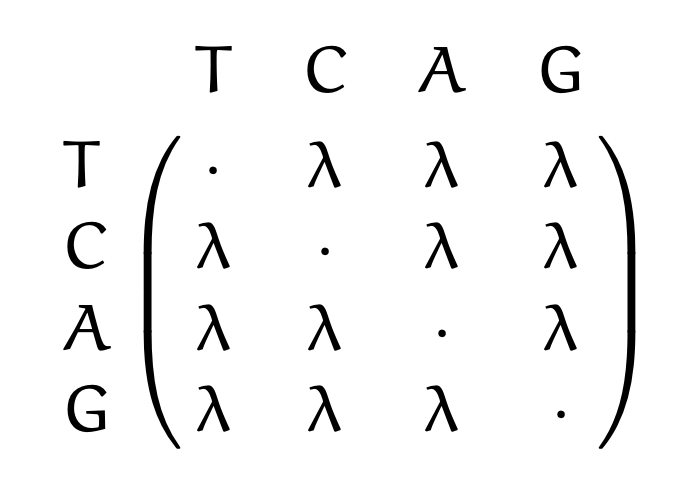
\includegraphics[width=0.5\linewidth]{js69.png}
\end{center}

\subsubsection{K80}
\begin{itemize}
    \item This model differentiates between transitions (T-C/A-G) and transversions. 
    \item 2 parameters
\end{itemize}

\begin{center}
    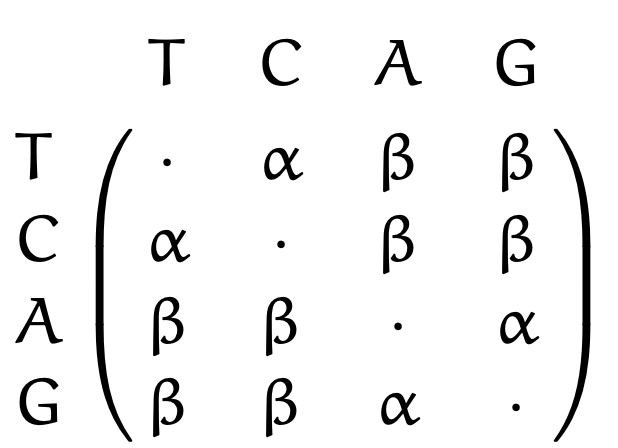
\includegraphics[width=0.5\linewidth]{k80.png}
\end{center}

\subsubsection{TN93}
\begin{itemize}
    \item Transitions between T/C happen with rate $\alpha_1 \times \pi$
    \item Transitions between A/G happen with rate $\alpha_2 \times \pi$
    \item Transversions happen with rate $\beta\times \pi$
    \item 3 + 3 ($\pi_x$) parameters 
\end{itemize}

\begin{center}
    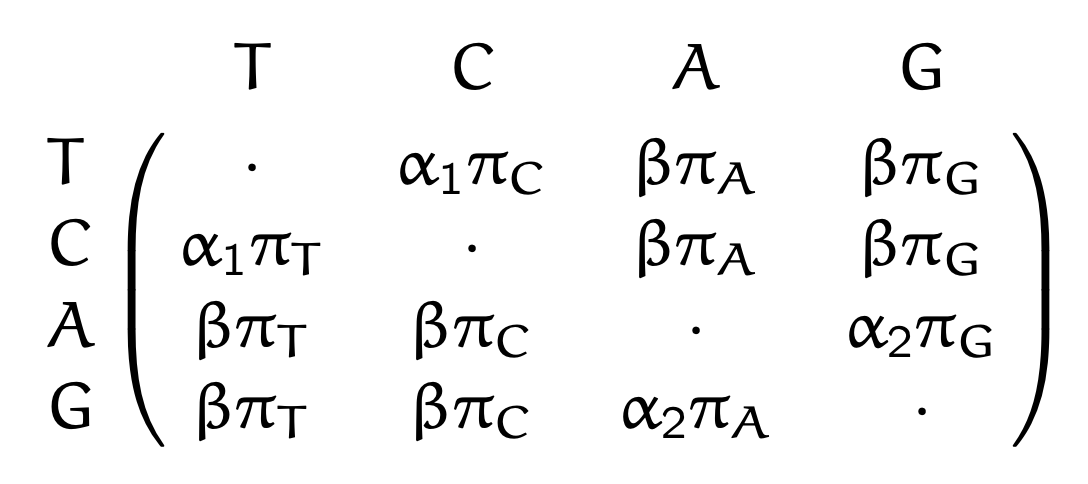
\includegraphics[width=0.7\linewidth]{tn93.png}
\end{center}

\begin{itemize}
    \item If $\alpha_1 = \alpha_2$, the model is named \textbf{HKY}
\end{itemize}

\subsubsection{GTR - Generalised Time Reversible}

\begin{itemize}
    \item[+] quite flexible
    \item[+] time-reversible
    \item[-] not completely general
    \item 6 + 3 ($\pi_x$) parameters 
\end{itemize}

\begin{center}
    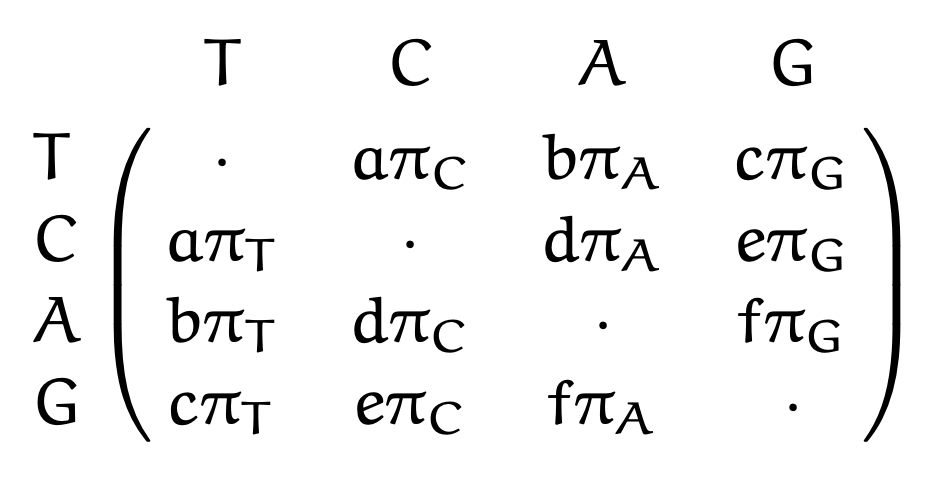
\includegraphics[width=0.7\linewidth]{GTR.png}
\end{center}
\subsubsection{UNREST}

\begin{itemize}
    \item Unrestricted model 
    \item Each substitution has a different rate
    \item[+] Most general model 
    \item[+] Other models are special cases of UNREST
    \item[-] Mathematically complicated to handle
    \item[-] Not time-reversible
    \item 12 parameters 
\end{itemize}

\begin{center}
    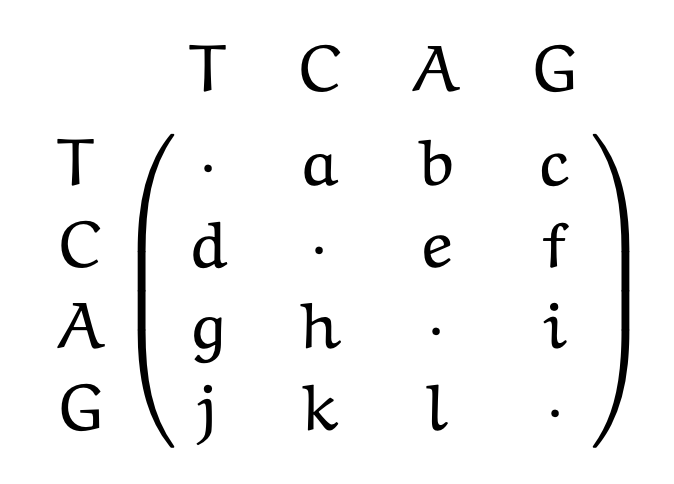
\includegraphics[width=0.5\linewidth]{unrest.png}
\end{center}

\subsection{Calculating Sequence Distance}
\subsubsection{Transition Probability Matrix}
\label{transprobmat}

Using the substitution rate matrix $Q$ we derive the transition probability matrix $P(t)$, which gives the probabilities of nucleotide $i$ changing to nucleotide $j$ in any time interval $t$.

\begin{center}
    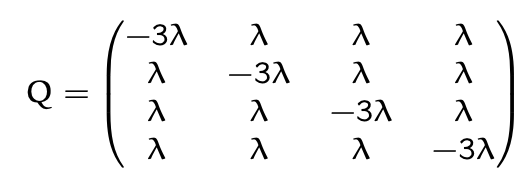
\includegraphics[width=0.5\linewidth]{substitutionratematrix.png}
\end{center}

$$P(t) = \text{e}^{Qt}$$

\begin{center}
    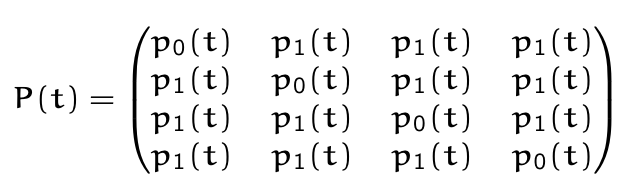
\includegraphics[width=0.7\linewidth]{transitionprobabilitymatrix.png}
\end{center}

\subsubsection{Stationary Distribution}

\begin{itemize}
    \item For $t \rightarrow \infty$ we reach a stationary distribution; where the transition probabilities tend towards their equilibrium frequencies.% (all $0.25$ under JC69). 
    \item Any long sequence will thus be composed of equal amounts of T,C,A and G at $t \rightarrow \infty$ under JC69. %(equilibrium frequency of $0.25$ for all nucleotides).
\end{itemize}

\subsection{Maximum Likelihood Estimators}
\begin{mdframed}[backgroundcolor=astral] 
    \textbf{Likelihood Function}\\
    Describes a hypersurface whose peak represents the combination of model parameter values that maximize the probability of drawing the obtained sample. 
\end{mdframed}

\begin{mdframed}[backgroundcolor=astral] 
    \textbf{Maximum Likelihood Estimator}\\
    Is an estimator of a model parameter that maximises the probability to obtain the observed results.
\end{mdframed}

\textbf{Example}: Estimate the probability that a die shows side 6. $\rightarrow$ The die is thrown $n = 100$ times and we obtained a 6 $x = 40$ times. 
\begin{itemize}
    \item Define probability of throwing a 6 $x$ times out of $n$ tries $\rightarrow$ Binomial-distribution, thus: $P = {n\choose x}p^x(1-p)^{n-x}$, where $p$ is the probability of throwing a 6
    \item We use this probability as our likelihood function and plug in the given values: $L(p;x) = {100\choose 40}p^{40}(1-p)^{60}$
    \item To find the maximum likelihood we calculate the first derivative of our likelihood function and set $L' = 0$ to find the maximum. 
    \item Transformations are sometimes applied to the likelihood function. e.g.: $l(p;x) = \log (L(p;x))$
    \item We estimate the probability by solving for $p$ and get $p = 0.4 \neq 1/6$
\end{itemize}

\subsubsection{Confidence Intervals}

Interval which tries to capture the uncertainty of a parameter estimate. 

\begin{mdframed}[backgroundcolor=astral] 
    \textbf{Confidence Interval}\\
    If a parameter is repeatedly estimated from realisations of the random experiment and the interval estimate for each realisation, we expect 95 \% of these intervals to contain the true parameter.
\end{mdframed}

Confidence intervals may be calculated on the basis of likelihood intervals.\\
Let $X$ be a random variable with a distribution parametrised in $\theta$. Based on collected data $x$ of a huge sample, the maximum likelihood estimation for the parameter is $\hat{\theta}$. Then, $2(l(\hat{\theta}) - l(\theta)) \sim \chi^2_k$
\begin{itemize}
    \item Determine the value of the log likelihood function in $\hat{\theta}$: $l(\hat{\theta};x)$
    \item Calculate $l(\hat{\theta};x) - 0.5\chi^2_{k,5\%}$; subtract half of the $5\%$ most extreme values according to the $\chi^2$-distribution
    \item Determine those $\theta$ values for which the the following holds: 
    $l(\theta;x) = l(\hat{\theta};x) - 0.5\chi^2_{k,5\%}$
\end{itemize}

\subsubsection{MLE for Sequence Distance}
The MLE framework can be used to derive a maximum likelihood estimation for the sequence distance under a JC69 model. 
We have the transition probability matrix as seen in subsection (\ref{transprobmat}) with:
\begin{align*}
    p_0(t) = \frac{1}{4} + \frac{3}{4}\text{e}^{-4\lambda t}\\
    p_1(t) = \frac{1}{4} - \frac{1}{4}\text{e}^{-4\lambda t}
\end{align*}
For two sequences of length $n$ with $x$ differences the probability that any one position is different is $p = 3p_1(t)$. We define $d = 3\lambda t$ as the expected distance in time $t$ and get for the probability that $x$ out of $n$ positions are different: \begin{align*}
L(d;x) = {n \choose x} p^{x}(1-p)^{n-x}=\\
{n \choose x}
\left(\frac{3}{4}-\frac{3}{4} e^{-\frac{4}{3} d}\right)^{x}\left(\frac{1}{4}+\frac{3}{4} e^{-\frac{4}{3} d}\right)^{n-x}
\end{align*}
\begin{itemize}
    \item We compute $l(d;x) = \log(L(d;x))$
    \item And calculate the first derivative and set it to zero $l'(d;x) = 0$
\end{itemize}

Which gives us the MLE of the JC69 distance: 
$$\hat{d} = -\frac{3}{4}\log\left(1-\frac{4x}{3n}\right)$$

\subsubsection{Example of JC69 MLE}

\begin{center}
    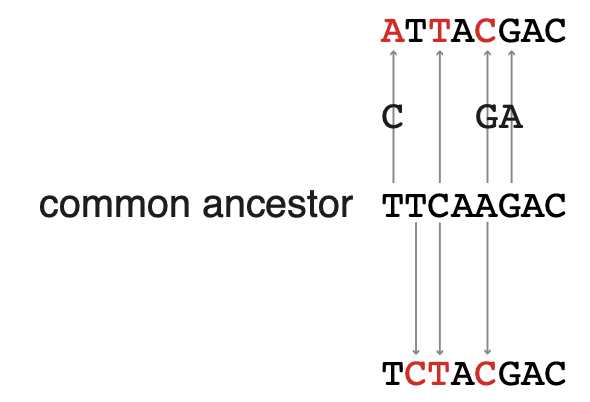
\includegraphics[width=0.5\linewidth]{mlejc69.png}
\end{center}

\begin{itemize}
    \item Length of gene: $n = 8$
    \item Differences between the two sequences: $x = 2$
\end{itemize}

$$\hat{d} = -\frac{3}{4}\log\left(1-\frac{4\times 2}{3\times 8}\right) = 0.3$$
Determine the $95 \%$ confidence interval for the given parameters. 

\subsection{Variable Substitution Rates}

\begin{itemize}
    \item Not all sites evolve at the same rate
    \item Mutation rates may vary across sites \item The acting selection in the phenotypic level exerts different evolutionary pressure on different sites
    \item Extend the existing models by replacing the constant rate by a $\Gamma$-distributed random variable
\end{itemize}

\subsection{Codon Substitution Models}
$N_d$ : number of nonsynonymous differences \newline
$S_d$ : number of synonymous differences (taking into account all possible ways from seq1 to seq2)
\newline
$N$ : number of nonsynonymous sites
\newline
$S$ : number of synonymous sites
\begin{itemize}
    \item Use $\frac{N_d}{N}$ and $\frac{S_d}{S}$ as $p$-distances
    \item Calculate $d_N$ and $d_S$ with their respective $p$-distance with respect to the chosen substitution model
    \item $\frac{d_N}{d_S}<1$ implies that nonsynonymous mutations occur less frequently than synonymous mutations (purifying selection)
    \item $\frac{d_N}{d_S}>1$ implies that nonsynonymous mutations occur more frequently than synonymous mutations (positive selection)
\end{itemize}
\section{Sequence Distance}
t
\section{Phylogenetic Inference}
There are three phylogenetic approaches
\begin{itemize}
   \item Phenetic approach
   \newline
     - Algoritmic approach (e.g. UPGMA algorithm)
    \newline
     - Optimality approach (e.g. Least squares methods)
   \item Cladistic approach
    \newline
     - Parsimony approach
   \item Mechanistic approach
    \newline
     - Maximum Likelihood approach
\end{itemize}
While phenetic approach give statistically consistent result (true tree returned if infinite amount of data available) cladistic approach is not.

\subsection{Phenetic approach}
\subsubsection{UPGMA algorithm}
\begin{itemize}
    \item Output an ultrametric tree (all sequences must be sampled at the same time)
    \item Assumes evolution according to a strict molecular clock
    \item The distances from the UPGMA tree might not be exactly the same as is the distance matrix
\end{itemize}

\subsubsection{Least squares method}
\begin{itemize}
    \item Uses an optimality criterion
    \item Tries to lower the difference between the distance of two sequences from the tree and the distance matrix
    \item Needs a tree topology to be proposed and then give the optimal branch lengths given the topology
\end{itemize}

\subsection{Cladistic approach}
\subsubsection{Parsimony method}
\begin{itemize}
    \item Tries to lower the number of mutations
    \item Considers every possible unrooted tree given sequences alignment and calculate the parsimony score for each of them
    \item Output the unrooted tree with minimal parsimony score
    \item Uses Fitch algorithm to speed up the process
    \item Statistically inconsistent (because of long branch attraction in the Felsenstein zone)
\end{itemize}

\section{Cladistic and ML Inference}
{\color{red} MISSING CONTENT PP5-6; Here starts PP7}

\subsection{Searching Tree Space}
To search the tree space for the maximum likelihood tree we need to propose different trees for evaluation. 
\begin{itemize}
    \item We propose different unrooted trees using various defined moves to alter the tree
    \item We propose trees with different branch lengths; thus we multiply each branch length by some factor
\end{itemize}
$\rightarrow$ We can then use "hill-climbing" strategies to find the ML tree

\subsubsection{Modifying Unrooted Trees}

\begin{itemize}
    \item \textbf{Nearest-Neighbour Interchange (NNI)}: Swap two subtrees of opposing sides of one branch. 
    \item \textbf{Suptree Pruning and Regrafting (SPR)}: Remove one random subtree and attach at a random position of the tree.
    \item \textbf{Branch swapping by tree bisection and reconnection (TBR)}: Cut the tree into two and reconnect at random by selecting branches on both trees and connecting the subtrees between them. 
\end{itemize}

\subsection{Model Testing}

Here we introduce methods for model selection and assessing the confidence of our parameters. 

\subsubsection{Likelihood Ratio Testing}

\begin{itemize}
    \item Consider two models: $H_0$ as a general model parameterised in $\theta_0$ and $H_1$ as a nested model parameterised in $\theta_1$.
    \item Derive the likelihood function for both models and the maximum likelihood estimators $\hat{\theta}_0$ and $\hat{\theta}_1$ for given dataset. 
    \item Compute if $2(\log L (\hat{\theta}_1) - \log L(\hat{\theta}_0))$ is in the $\alpha$ tail of $\chi_{df}^2$, then reject the null model $H_0$   
\end{itemize}

\begin{mdframed}[backgroundcolor=astral] 
    \textbf{Likelihood Ratio Test}\\
    Is used to assess the goodness of fit of two models based on the ratio of their likelihoods. One model is found by maximizing the likelihood over the whole parameter space while the other is evaluated under some constraints. If the constraint (hypothesis) is supported by the data the likelihoods should not differ significantly.
\end{mdframed}

\subsubsection{Testing Non-Nested Models}

\textbf{Akaike Information Criterion (AIC)}: Used for testing non-nested models:
$$\text{AIC} = -2\log L_i(\hat{\theta}_i) + 2p_i$$
where $p_i$ is the number of parameters and $L_i$ the likelihood function of model $i$.

\begin{itemize}
    \item Calculate the AIC for each model
    \item Choose the model with the lowest AIC; thereby minimizing the Kullback-Leibler distance to the true model  
\end{itemize}

Rules of thumb for multiple model comparisons: 
\begin{itemize}
    \item AIC $\leq$ 1-2 + minimum $\rightarrow$ substantial support, should receive consideration in inference
    \item AIC $\leq$ 4-7 + minimum $\rightarrow$ low support
    \item AIC $\geq$ 10 + minimum $\rightarrow$ essentially no support
\end{itemize}

\subsubsection{Confidence Intervals}

Each parameter value which is not rejected based on the likelihood ratio test at the $0.05$ level is within the $95\%$ interval.
$\rightarrow$ Use the strategy as introduced before.
\begin{itemize}
    \item Determine the value of the log likelihood function in $\hat{\theta}$: $l(\hat{\theta};x)$
    \item Calculate $l(\hat{\theta};x) - 0.5\chi^2_{k,5\%}$; subtract half of the $5\%$ most extreme values according to the $\chi^2$-distribution
    \item Determine those $\theta$ values for which the the following holds: 
    $l(\theta;x) = l(\hat{\theta};x) - 0.5\chi^2_{k,5\%}$
\end{itemize}

\subsubsection{Bootstrapping}
\begin{itemize}
    \item Sample $m$ sites at random with replacement
    \item Infer a phylogeny based on the new data
    \item Repeat this procedure many times 
\end{itemize}

\begin{center}
    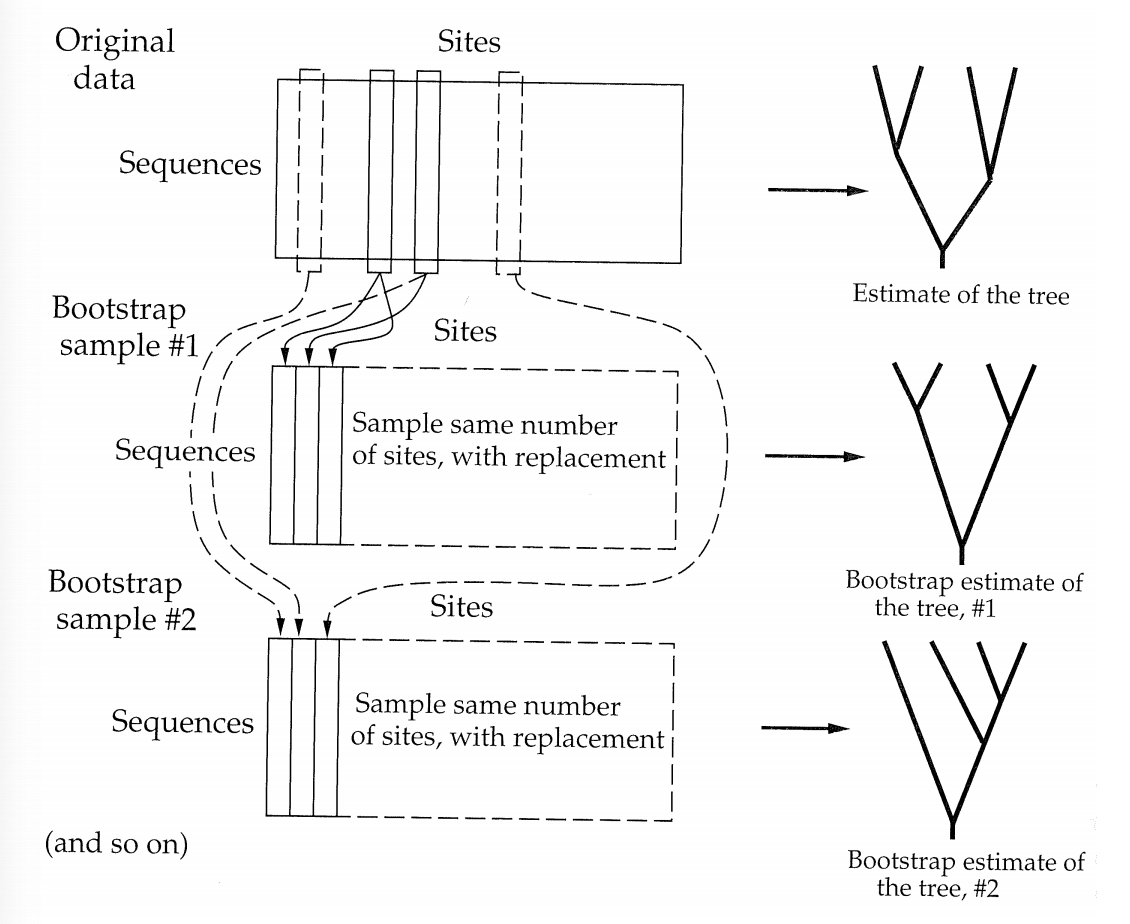
\includegraphics[width=1\linewidth, angle=0.6]{bootstrapping.png}
\end{center}

\subsection{Overview of ML Inference}

\begin{enumerate}
    \item Infer a ML tree 
    \begin{itemize}
        \item Felsenstein's pruning algorithm for each tree and branch length
        \item Choose the tree with branch lengths that optimize the likelihood
        \item Do this for each substitution model and calculate its AIC
    \end{itemize}
    \item Determine the substitution model and tree with highest support using AIC
    \item Determine the confidence interval for the substitution model parameters based on the likelihood ratios
    \item Determine the confidence in your maximum likelihood tree using bootstrapping
\end{enumerate}

\section{Comparative Methods}

\subsection{Comparing Discrete Characters}

Example: We want to know whether eye and hair color are correlated. 

\begin{center}
    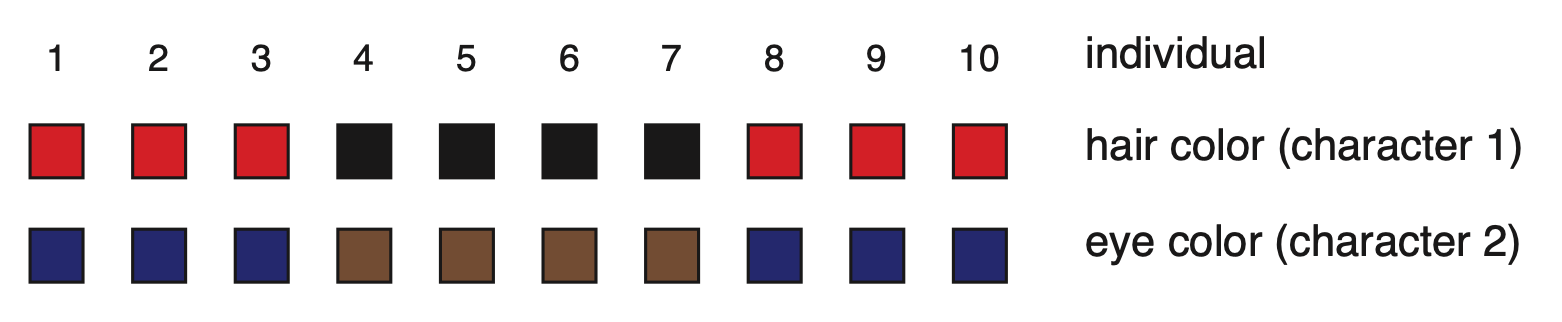
\includegraphics[width=1\linewidth, angle=0.0]{compdischar.png}
\end{center}

To test whether there is a true correlation we perform Fisher's exact test.\\
$H_0$: Having brown eyes is equally likely among red- and black-haired individuals.\\

\begin{tabular}{|l|l|l|}
\hline
\textbf{hair/eyes} & \textbf{brown} & \textbf{blue} \\ \hline
\textbf{red}       & 0              & 6             \\ \hline
\textbf{black}     & 4              & 0             \\ \hline
\end{tabular}

Evaluating the contingency table above yields the following. 
{
\footnotesize
\begin{align*}
P(red/brown) =& \frac{(RBr\ in\ R)\times (BlBr\ in\ Bl)}{Br\ in\ All}\\
=& \frac{{6\choose 0}{4\choose 4}}{{10\choose 4}} = 0.0048 < 0.05
\end{align*}
}
Thus we reject the hypothesis of independent character evolution on the 0.05 significance level, indicating that there is a correlation. 

\textbf{Caveat}: We should consider that there may be a bias due to the relatedness of the individuals. Fisher's exact test assumes independence which may not be given here.\\

\subsubsection{Reformulated Fisher's Test}

Thus we reformulate our problem: \textbf{Is the change of characters on the branches correlated?}

\begin{center}
    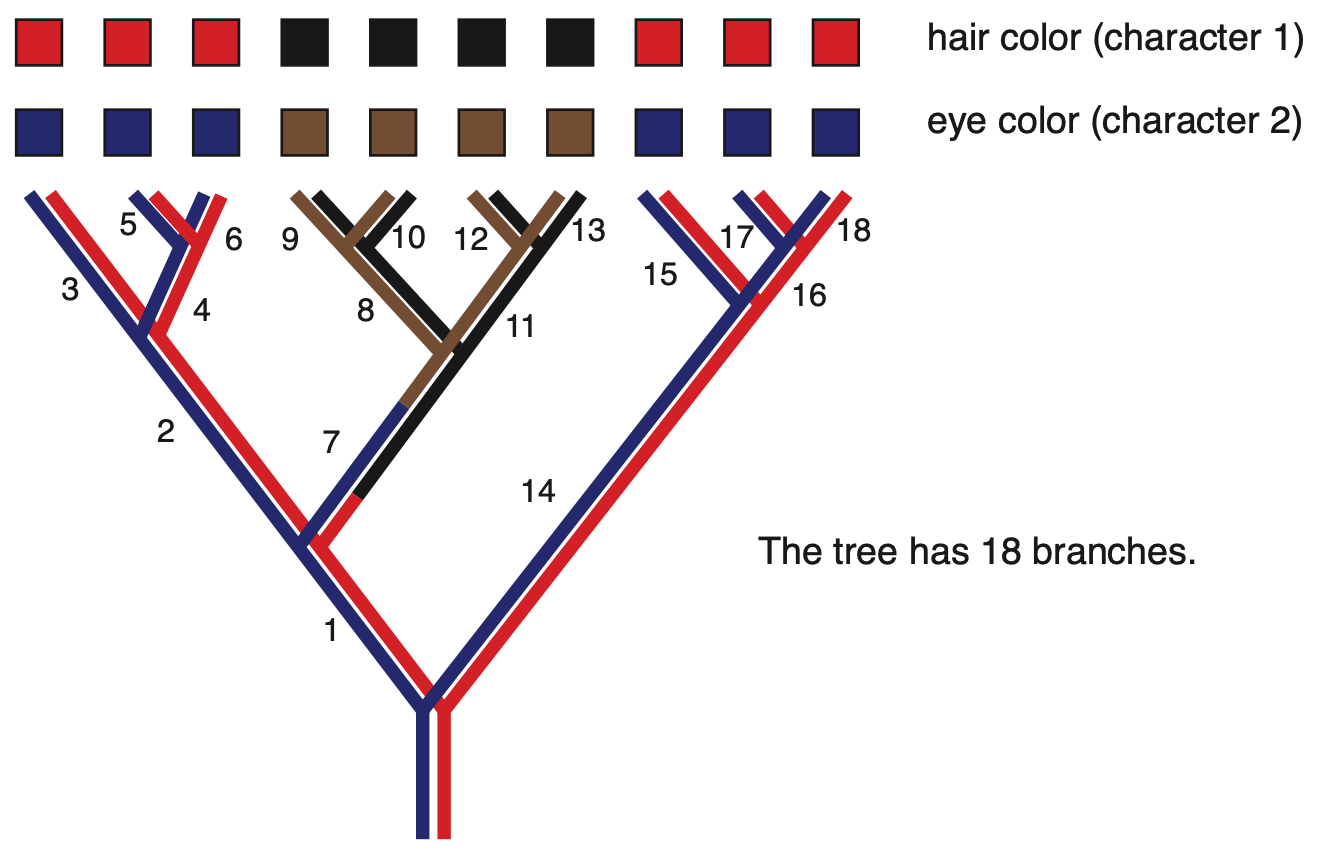
\includegraphics[width=1\linewidth, angle=0.0]{compdischarphylo.png}
\end{center}

$H_{0, new}$: The character changes are equally likely on every branch.\\ 

\begin{tabular}{|l|l|l|}
\hline
\textbf{hair/eyes} & \textbf{yes} & \textbf{no} \\ \hline
\textbf{yes}       & 1              & 0             \\ \hline
\textbf{no}     & 0              & 17             \\ \hline
\end{tabular}\\

This contingency table summarizes on how many branches we have a change in either the hair color, the eye color or both. Here we have \textbf{one} branch with a change in both and \textbf{17} branches with no change.\\

The probability for one branch on which both the hair and eye color changes ($E$) is under $H_{0, new}$:

\begin{align*}
    P(E|H_{0,new}) =& \frac{{1\choose 1}{17\choose 0}}{{18\choose 1}} = 0.05555 > 0.05
\end{align*}

Neglecting the phylogenetic background can lead to false conclusions on correlations between characters, because of non-independence of species data points as a result of shared ancestry.\\

Here we do not consider differences in branch length, but these are important as changes are more likely to happen on longer branches. 

\subsection{Comparing Continuous Characters}

We now switch our focus from discrete characters (e.g. color) to continuous phenotypic characters (e.g. height, weight, virulence). 

\subsubsection{Linear Regression on Phylogenies}

We cannot use linear regression models two compare two characters which evolved on a phylogeny as we cannot distinguish between correlations and clade effects. 

\begin{center}
    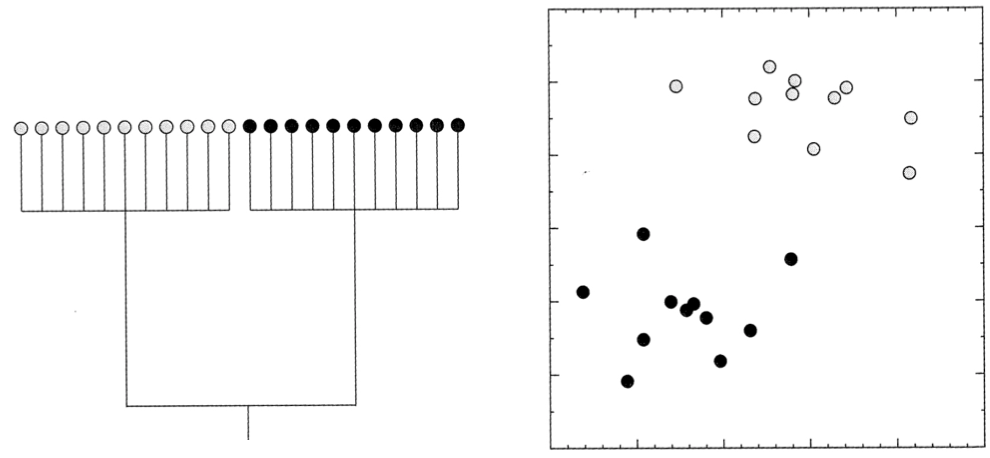
\includegraphics[width=1\linewidth, angle=0.0]{phyloregress.png}
\end{center}

When characters evolve on a tree:

\begin{itemize}
    \item ...they share common evolutionary history and are not independent realisations
    \item ...the variance/error added by Brownian motion is not equally distributed 
\end{itemize}

Thus the prerequisites for linear regression (see: {\color{astral}Linear Regression}) are not given.  
\subsubsection{Brownian Motion}

Brownian motion is a Wiener process and thus follows four conditions: 

\begin{itemize}
    \item $W_0$ = 0, the process start in $0$
    \item $W_t$ is almost surely continuous: $P(W_t$ continuous $) = 1$  
    \item $W_t$ has independent increments (memorylessness): For $0 \leq s_1 \leq t_1 < s_2 \leq t_2$, $(W_{t_1} - W_{s_1})$ and $(W_{t_2} - W_{s_2})$ are independent 
    \item For $0 \leq s \leq t$, the $W_t - W_s \sim N(0,\sigma^2(t-s))$
\end{itemize}

There are analogies between models for evolution on discrete and continuous character space.
\begin{center}
    \begin{tabular}{|l|l|}
\hline
\textbf{discrete}                                                                         & \textbf{continuous}                                                                   \\ \hline
\begin{tabular}[c]{@{}l@{}}probability\\ to visit any\\ state\end{tabular}                & \begin{tabular}[c]{@{}l@{}}probability\\ density on \\ state space\end{tabular}       \\ \hline
\begin{tabular}[c]{@{}l@{}}memory-\\ lessness due\\ to Markov-\\ chain model\end{tabular} & \begin{tabular}[c]{@{}l@{}}memory-\\ lessness due\\ to Brownian\\ motion\end{tabular} \\ \hline
\begin{tabular}[c]{@{}l@{}}transition\\ probabilities\\ scale with \\ time\end{tabular}   & \begin{tabular}[c]{@{}l@{}}variance\\ scales \\ with \\ branch \\ length\end{tabular} \\ \hline
\end{tabular}
\end{center}

Given a phylogeny we can apply a Brownian motion model to evolve a continuous character. 

\begin{center}
    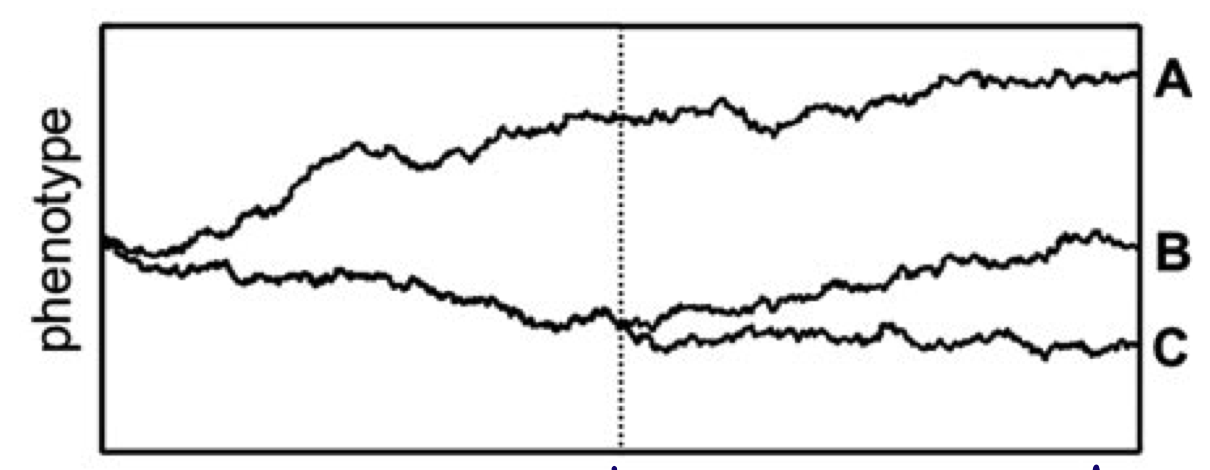
\includegraphics[width=1\linewidth, angle=0.0]{brownphyl.png}
\end{center}

\begin{mdframed}[backgroundcolor=astral] 
    \textbf{Linear Regression}\\
    Determine dependency of a variable $Y$ in another variable $X$. We measure $Y$ and $X$ for $n$ independent realizations and fit a regression model to the data. The observations need to be:
    \begin{itemize}
        \item independent
        \item have the same (normally) distibuted errors
    \end{itemize}
    
    Then we have the model: 
    
    $$y_i = \beta x_i + b + \epsilon, \text{ where } \epsilon \sim N(0, \epsilon^2)$$
    
    This is fit using a least squares method and the goodness of fit is estimated by $R^2$. An $R^2$ of $1$ indicates a perfect fit. 
\end{mdframed}

\subsubsection{Constructing Independent Variables}

One method to overcome interdependencies of the evolutionary trait is the contrast method.\\ 
Suppose we have the following phylogeny with four species; traits $X_1^j$ and $X_2^j$ are not independent as they share the evolutionary lineages $t_6$ and $t_7$.  
\begin{center}
    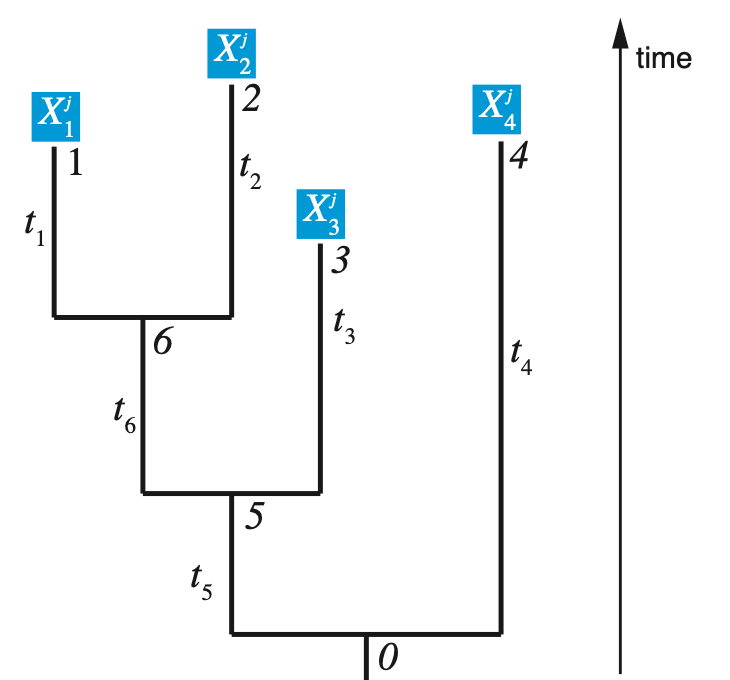
\includegraphics[width=0.6\linewidth, angle=0.0]{depchar.png}
\end{center}

We now consider the contrasts of the characters instead of the characters. As these are independent. 

\begin{center}
    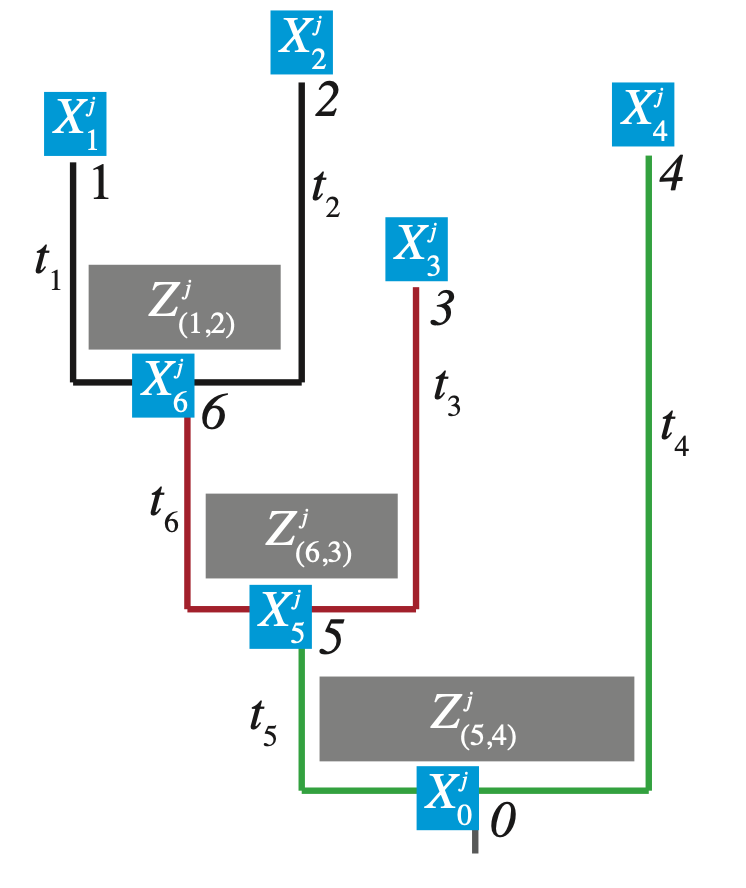
\includegraphics[width=0.6\linewidth, angle=0.0]{indepchar.png}
\end{center}

We now calculate the values of the independent contrasts and their variances. 

\begin{align*}
    z^j_{(1,2)} =& x_1^jx_2^j\\
    z^j_{(6,3)} =& x_6^jx_3^j\\
    z^j_{(5,4)} =& x_5^jx_4^j
\end{align*}

We assume \textbf{character evolution according to Brownian motion}. And we consider that we observe tip values but have to estimate values of internal nodes.\\

In order to calculate the variance we apply the following formula.

$$Var[\alpha X + \beta Y] = \alpha ^2 Var[X] + \beta ^2 Var[Y] + 2\alpha \beta Cov[X,Y]$$

The branch length at cherries can easily be calculated. The variance is proportional to the branch length between the two external nodes. 

\begin{align*}
    Var[X_1^j] = \sigma ^2 (t_1+t_6+t_5)\\
    Var[X_2^j] = \sigma ^2 (t_2+t_6+t_5)\\\\
    Var[Z^j_{(1,2)}] = Var[X_1^j-X^j_2] = \\
    Var[X_1^j] + Var[X_2^j] - 2 Cov[X_1^j,X_2^j]\\
    = \sigma^2 (t_1+t_6+t_5+t_2+\\t_6+t_5-2(t_6+t_5))\\
    = \sigma ^2 (t_1 + t_2)
\end{align*}

\textbf{Contrasts at Internal Nodes}\\

We want to calculate $Z_{(i,l)} = X_i - X_l$ and $Var[Z_{(i,l)}]$
To calculate the values at the internal nodes we have: 

$$X_i = \frac{t_n}{t_m+t_n}X_m + \frac{t_m}{t_m+t_n}X_n$$

and the corresponding variances: 

\begin{align*}
Var[X_i] = Var[\frac{t_n}{t_m+t_n}X_m +\\ \frac{t_m}{t_m+t_n}X_n] =\\
\sigma ^2 \left(\frac{t_mt_n}{t_m+t_n}+ t_i + t_k + ...\right)
\end{align*}

\textbf{Normalisation of Contrasts}
To make contrasts comparable to each other they all need to have the same variance. Thus we normalise all contrasts in a last step.\\

Given the contrast $Z^j_{(i,l)}$ with variance $Var[Z^j_{i,l}] = \sigma^2c_{z^j_{(i,l)}}$ we know that $Var(\alpha X) = \alpha ^2 Var(X)$. Thus we can replace the contrasts by the following. 

\begin{align*}
    Z^j_{(i,l), norm} = \frac{Z^j_{(i,l)}}{\sqrt{c_{z^j_{(i,l)}}}}
\end{align*}

With $Z^j_{(i,l), norm} \sim N(0, \sigma ^2)$, the contrasts may now be used for linear regression analysis. 

\section{Phylodynamic Inference and Birth Death Models}

Phylodynamic trees encode past macroevolutionary dynamics. \\%; in macroevolution ??? are the unit of focus.\\
We define the following terms.
\begin{itemize}
    \item \textbf{Molecular Evolution}: Genetic makeup of species changes through time 
    \item \textbf{Phylogenetics}: Phylogeny displays the relationship between species
    \item \textbf{Phylodynamics}: Dynamics of population; speciation and extinction processes 
\end{itemize}

In epidemiology we these terms as follows. 

\begin{itemize}
    \item \textbf{Evolution}: Pathogen is evolving trough time
    \item \textbf{Phylogenetics}: The phylogeny display the transmission history
    \item \textbf{Phylodynamics}: Transmission and becoming non-infectious
\end{itemize}

In this context we look at the basic reproductive number $R_0$, which is the average number of secondary infections caused by a single infected individual.\\

\textbf{Applications}: Phylogenetic modelling is used outside its traditional realm. 
\begin{itemize}
    \item \textbf{Immunology}: B cells are the unit of evolution 
    \begin{itemize}
        \item Phylogeny displays B cell differentiation trough somatic hypermutation
        \item Population dynamics are represented by the B cell generation and loss
    \end{itemize}
    \item \textbf{Cancer}: Cells are the unit of evolution 
    \begin{itemize}
        \item Phylogeny displays relationship of different cancer cells and healthy cells 
        \item Population dynamics is represented by the spread an loss of cell types 
    \end{itemize}
    \item \textbf{Languages}: Languages are the unit of evolution 
    \begin{itemize}
        \item Phylogeny displays language evolution
        \item Population dynamics is the gain and loss of languages
    \end{itemize}
\end{itemize}

\subsection{Phylodynamics}

Population dynamics models the birth and death of individuals (species, infected hosts, B cells, cancer cells and languages). Phylodynamics aims to understand and quantify the population dynamics based on a phylogenetic tree. 

\subsubsection{Population Dynamic Models}

We look at a linear birth-death process which models the reproduction and death of individuals with the following simple model. 

\begin{center}
    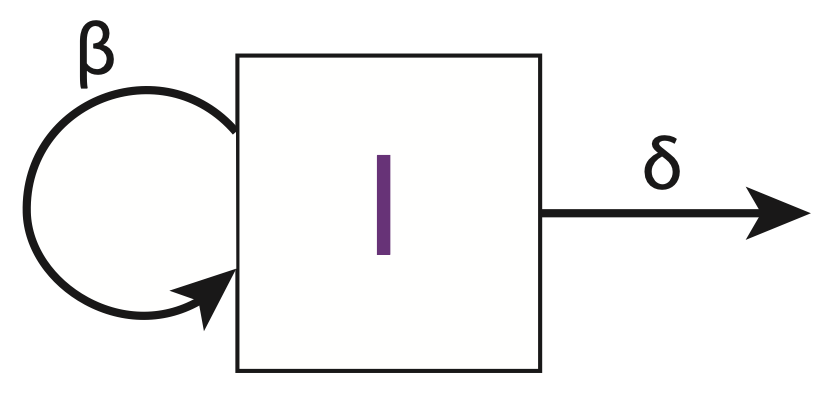
\includegraphics[width=0.6\linewidth, angle=0.0]{birthdeath.png}
\end{center}

\begin{itemize}
    \item $\beta$: The rate of birth of new individuals per individual in $I$
    \item $\delta$: The rate of death per individual in $I$
\end{itemize}

Thus if we consider the fate of one individual we see that. 
\begin{itemize}
    \item The probability of giving birth to another individual in a very small time step $\Delta t$ is $\beta \Delta t$.
    \item The probability of dying in a very small time step $\Delta t$ is $\delta \Delta t$
    \item The waiting time to the first birth or death event is exponentially distributed with parameter $\beta + \delta$, as the minimum of two exponentially distributed random variables with rates $r_1$, $r_2$ is exponentially distributed with rate ($r_1 + r_2$). 
\end{itemize}

Thus if we consider the waiting time of $N$ individuals we find that.
\begin{itemize}
\item The waiting time of the first event is exponentially distributed with parameter $N(\beta + \delta)$
\end{itemize}

The following diagram illustrates the full population dynamics of a birth-death process which starts with one individual and is stopped after time T. 

\begin{center}
    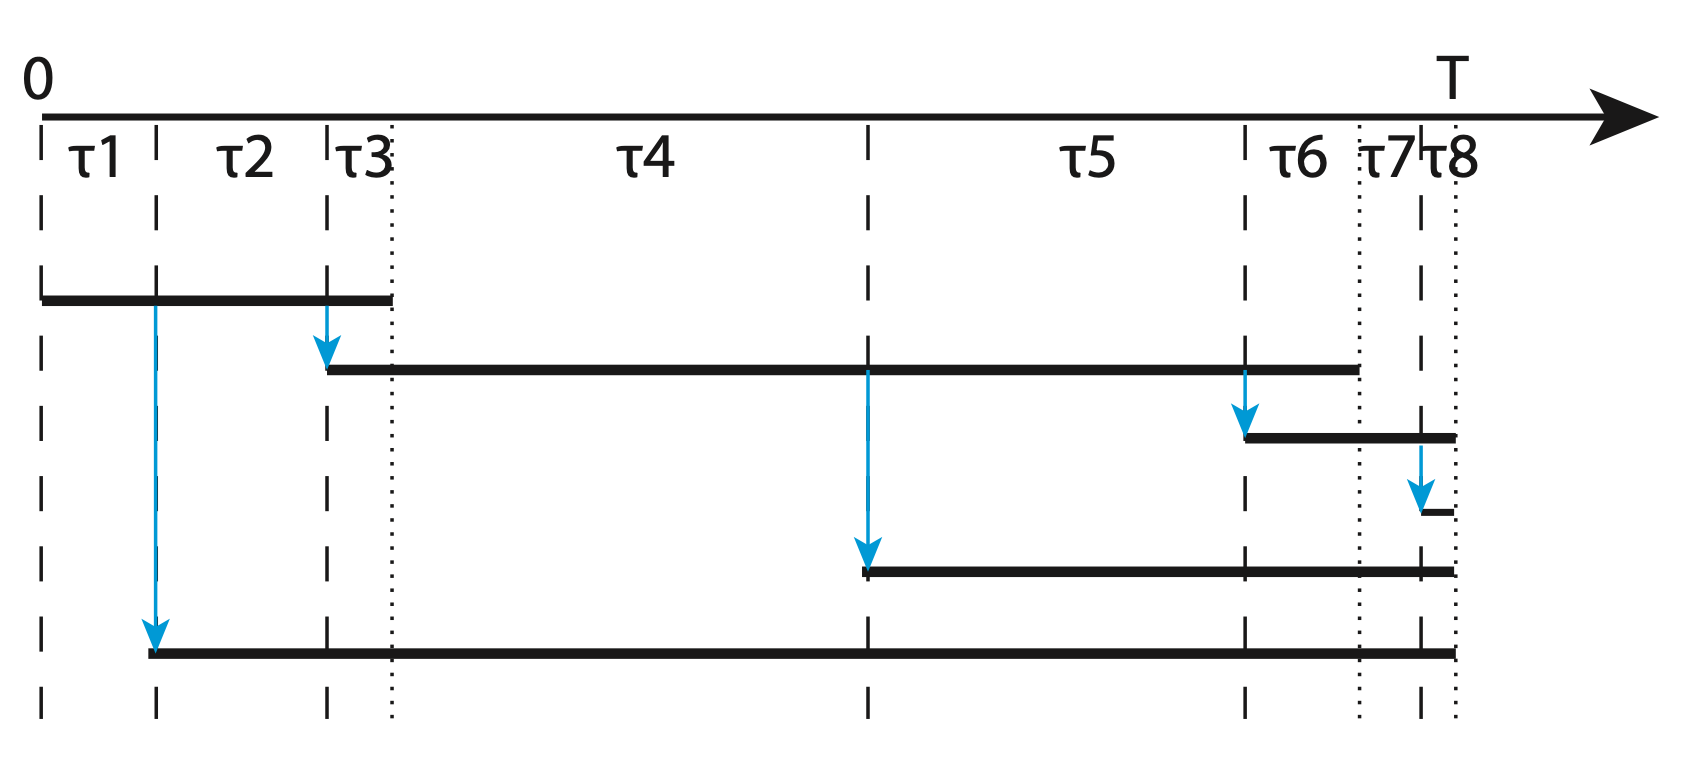
\includegraphics[width=1\linewidth, angle=0.0]{bddiagram.png}
\end{center}

\subsection{Phylodynamic Models}

A phylodynamic model adds a sampling process of individuals to the population dynamics. In a simple model we have the following. 

\begin{itemize}
    \item Birth rate $\beta$
    \item Death rate $\delta$
    \item Process duration $T$
    \item Extant tip sampling probability $\rho$
    \item Extinct tip sampling probability $\phi$
\end{itemize}


If we assume $\rho = 1$, $\phi = 0$ in the context of macro-evolution that means that we do not sample from fossils but only from extant (species still living today) species. The subtree of the complete population tree connecting the sampled individuals and ignoring parent-children labels, is called the phylogenetic tree. This is displayed in the lower part of the following figure, where the parent-child information is removed and only extant species are shown. %($\rho = 1$, $\phi = 0$). 


\begin{center}
    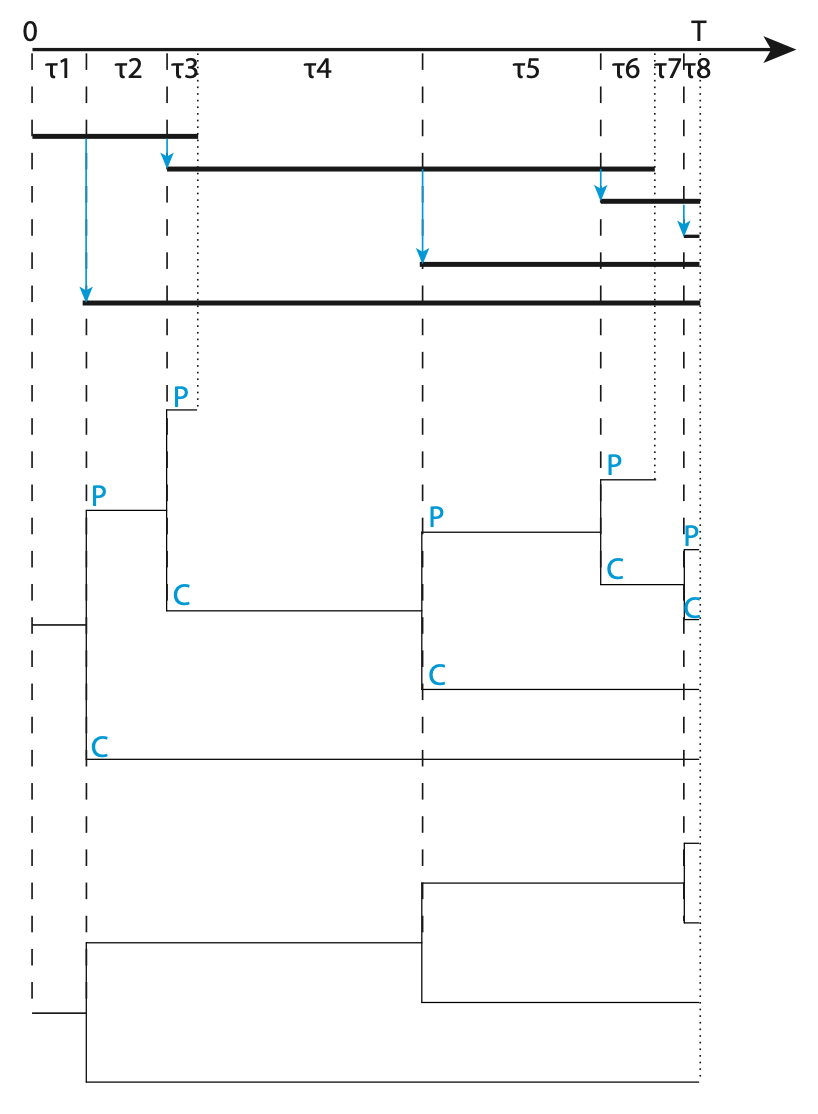
\includegraphics[width=0.8\linewidth, angle=0.0]{extanttree.png}
\end{center}

We introduce the lineage through time (LTT) plot here, it indicates the number of surviving lineages trough time. The dashed blue line is the LTT plot of the complete tree and includes population size through time while the red line only shows the number of surviving lineages. 

\begin{center}
    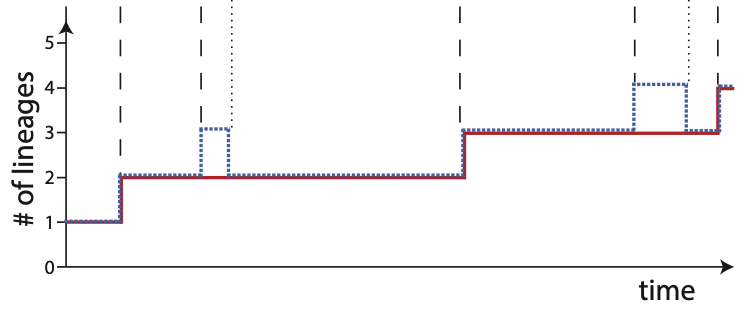
\includegraphics[width=0.8\linewidth, angle=0.0]{ltt.png}
\end{center}

LTT plots provide a method of estimating parameters of birt death models. The following plot shows a large number of realization of a birth-death model simulation. The simulation was run with $T = 50, \beta > \delta$. If $\beta < \delta$ the population would decrease on average and most trees would rapidly go extinct. We plot the average over all LTT for the phylogenetic trees ({\color{red} red}), the average over all LTT plots for the complete trees ({\color{blue} blue}) and the average total population size over all realizations (complete and extinct trees) (black).

\begin{center}
    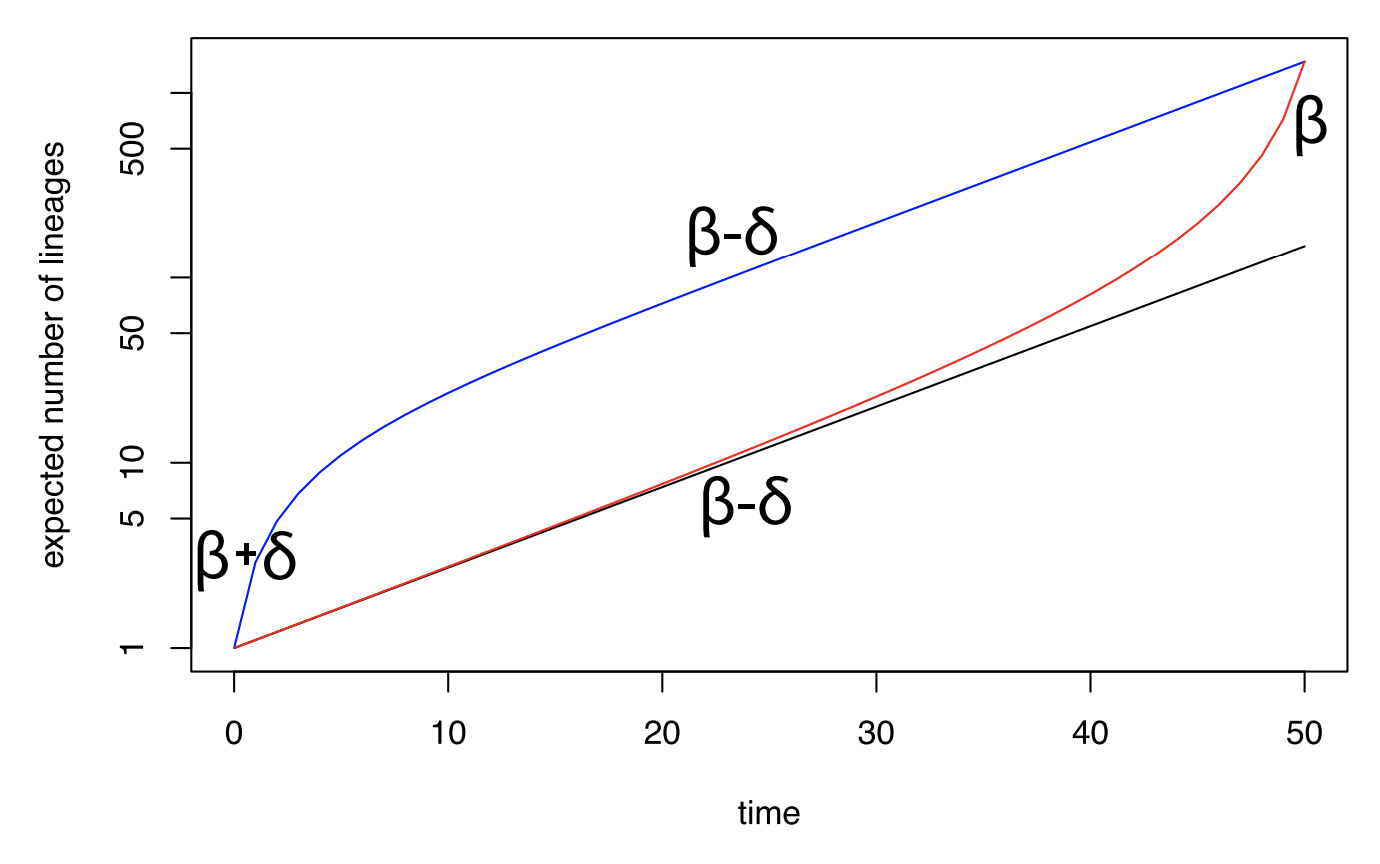
\includegraphics[width=1\linewidth, angle=0.0]{lttavg.png}
\end{center}

At the start of the complete LTT plot we see an increased slope, this effect is called "push-of-the-past"; the increased slope at the end of the phylogenetic LTT plot is called "pull-of-the-present". 

\begin{itemize}
    \item \textbf{Average Total Population Size}: The average total population size through time has the constant slope $\beta - \delta$ on the log scale, corresponding to the average total population size of $\text{e}^{(\beta - \delta)t}$ at time $t$.
    \item \textbf{Complete LTT Plot}: The complete LTT plot goes through a period of accelerated growth at the beginning of the process, before growing exponentially at rate $\beta - \delta$. This may be explained by the fact that the complete LTT plot only includes populations that survive to the present. Thus we expect populations that grow slowly at the start to be less likely to survive to the end of the process and are thus not included in the complete LTT plot (push-to-the-past).
    \item \textbf{Phylogenetic LTT Plot} The phylogenetic LTT plot grows exponentially with rate $\beta - \delta$ until the present when the growth accelerates to exponential growth with rate $\beta$. This may be explained by the fact that lineages appearing close to the end of the process have not enough time to go extinct and are thus more likely to be sampled.
\end{itemize}
\subsubsection{Parameter Estimation with LTT}

The following figure indicates how the paramters $\beta$ and $\delta$ can be determined from the phylogenetic LTT plot. The stars indicate a branching event at time $t$ with the number of lineages after the event on the $y$-axis. We fit a line to the initial slope and find $\beta - \delta$ and to the recent slope to find $\beta$.\\

\begin{center}
    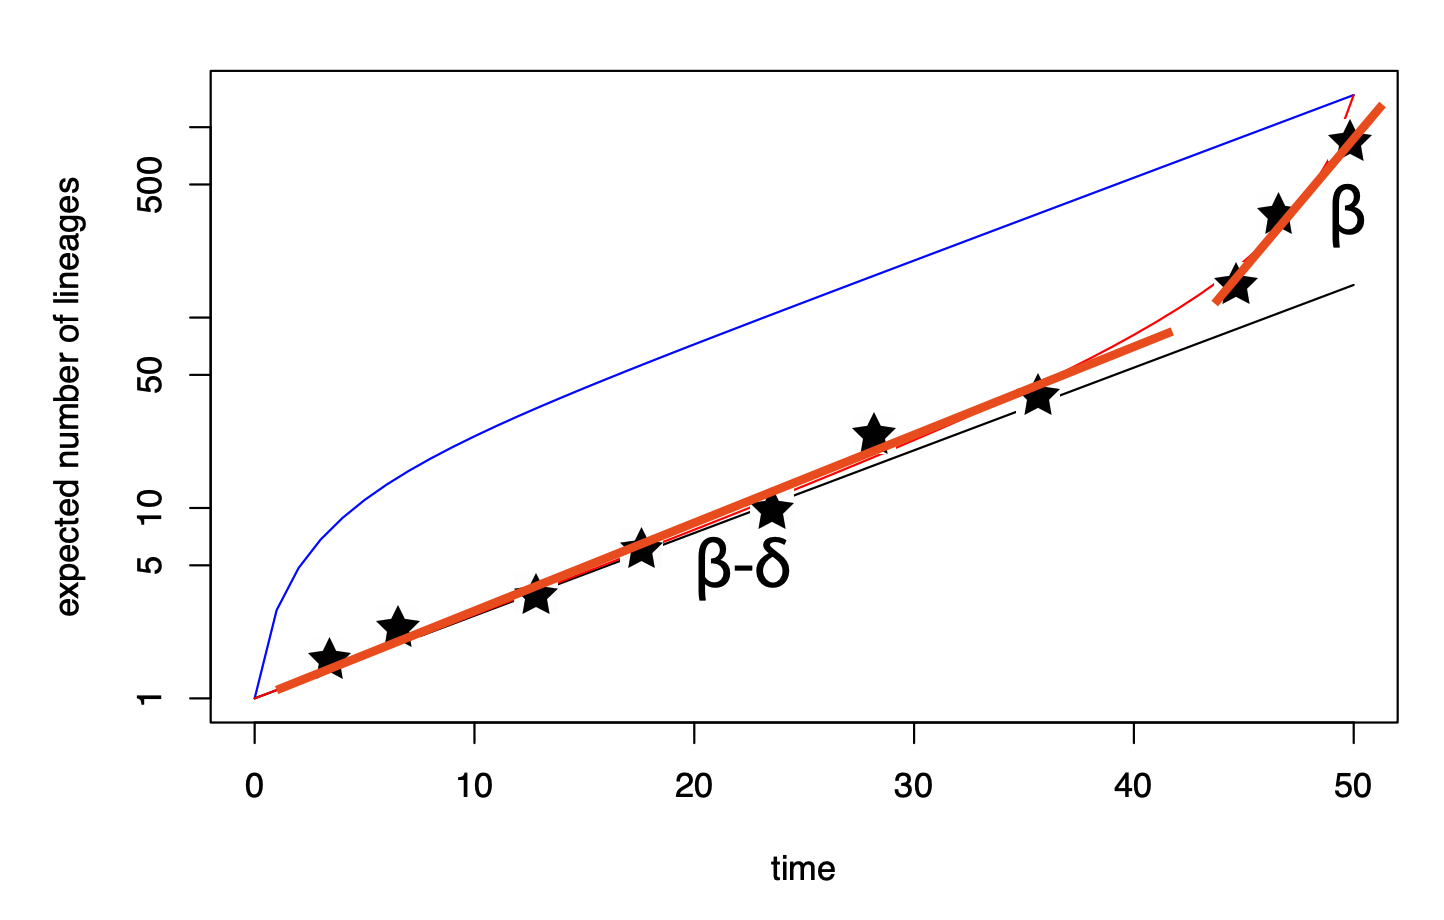
\includegraphics[width=1\linewidth, angle=0.0]{lttregression.png}
\end{center}

However estimating parameters of the birth-death model in this manner is problematic.
\begin{itemize}
    \item The variance in the timing of the next branching event (next star) decreases with increasing population size. Thus a classic linear regression assuming the same variance for each data point (homoscedasticity) is not valid. 
    \item The time transition between the two phases of the curve is unclear. This poses the difficulty of deciding where to place the cutoff between the first and second regression line. 
\end{itemize}

\subsubsection{Probability Density of a Tree}

We recall that in phylogenetics we calculate the phylogenetic tree by evaluating the following likelihood function. 

$$L(T,Q;D) = P(D|T,Q)$$

Where $T$ is the phylogenetic tree, $Q$ is the substitution rate matrix and $D$ is the sequence alignement.\\

In phylodynamics we want to compute the phylodynamic likelihood which is defined as follows. 

$$L(\eta = (\beta, \delta, T, \rho, \psi, r); T) = P(T|\eta)$$

Where $T$ is the phylogenetic tree and $\eta$ summarizes the birth-death parameters.\\

We use a maximum likelihood approach with assumption of complete extant sampling (no fossil sampling), thus we have $\rho = 1,$ $\psi = 0$. We start by deriving the likelihood of a single individual to leave $0$ or $1$ offspring after time $t$.\\

The probability that no surviving individuals remain after time $t$ if we start with one individual is abbreviated as $p(0|t)$. We consider very small timesteps ($\Delta t$) during which only one event occurs. During this timestep for a single individual a death event happens with probability $\delta \Delta t$ and a birth event happens with probability $\beta \Delta t$. With probability $1-(\beta + \delta)\Delta t$ no event occurs. We derive the differential equation for $p(0|t)$ below. 

\begin{align*}
    p(0|t+\Delta t) =\\ \underbrace{(1- (\beta + \delta)\Delta t)p(0|t)}_{\text{No event}} + \underbrace{\delta \Delta t}_{\text{Death event}} + \underbrace{\beta \Delta t p (0|t)^2}_{\text{Birth event}}
\end{align*}

\begin{center}
    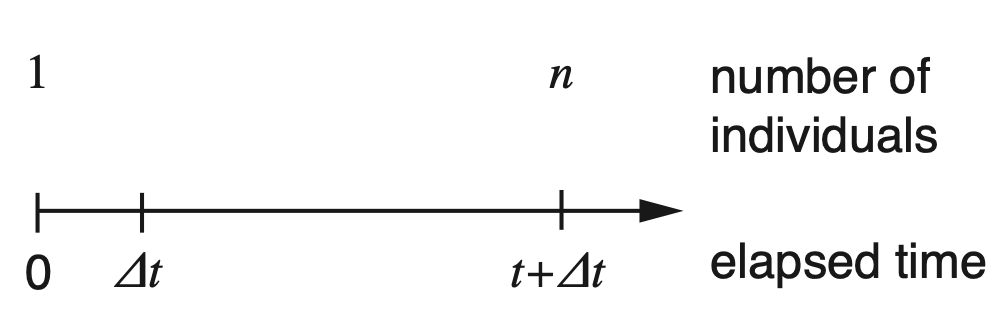
\includegraphics[width=1\linewidth, angle=0.0]{exprob.png}
\end{center}

The events are derived as follows. 

\begin{itemize}
    \item \textbf{No event}: We have probability $1-P(\text{Any event happens in time} \ \Delta t)$ that no event occurs in the time step $[0, \Delta t]$, to derive the probability that we have extinction we multiply with the probability of one individual dying out ($p(0|t)$). 
    \item \textbf{Birth}: We have the probability $\beta \Delta t$ that a birth happens times the probability that both these individuals die out ($p(0|t)^2$). 
    \item \textbf{Death} We have the probability $\delta \Delta t$ for a death event, in this case the probability for extinction is one as no individual remains. 
\end{itemize}

We rearrange the equation and get. 

\begin{align*}
    \frac{p(0|t+\Delta t)-p(0|t)}{\Delta t} =\\
    -(\beta + \delta)p(0|t) + \delta + \beta p(0|t)^2
\end{align*}

When we take the limit $\Delta t \rightarrow 0$, the following remains. 

$$\frac{d}{dt}p(0|t) = -(\beta + \delta) p (0|t) + \delta + \beta p(0|t)^2$$

With the initial condition of $p(0|0) = 0$ we solve the differential equation to get this. 

$$p(0|t) = \frac{\delta(1-e^{-(\beta - \delta)t})}{\beta-\delta e^{-(\beta -\delta)t}}$$

We extend the equation to the probability of $n$ surviving lineages after time $t$ and get the following after [Kendall et al., 1948]. 

$$p(1|t) = e^{-(-\beta - \delta)t}(1-p(0|t))^2$$
$$p(n|t) = p(1|t)\left(\frac{\beta}{\delta}p(0|t)\right)^{n-1}, \text{ for } n\geq 2$$

\textbf{Proof}\\

We prove the equation for $p(1|t)$ and write the following. 

$$\frac{d}{dt}p(1|t) = -(\beta + \delta)p(1|t) + 2\beta p(1|t)p(0|t)$$
The factor of two accounts for either one of the descendants of the birth event leading to a surviving individual at time $t$.
We evaluate both sides of the equation using $p(1|t) = e^{-(\beta -\delta)t}(1-p(0|t))^2$, thus showing that this function is a solution to the differential equation.\\

Solving the equation then leads to the following expression. 

$$p(1|t) = (1-p(0|t))(1-\frac{\beta}{\delta}p(0|t))$$
\subsubsection{Expansion of the Model to a Tree}

We assume that the time in this model is measured as age relative to the present, thus $t = 0$ is the present. We spilt the calculation into multiple sub-problems using dynamic programming. So let $p(x_0, x_1)$ be the probability density for a branch of length $x_0 - x_1$ extending from an individual at time $x_0$ in the past. Then, the probability density of a tree $T$ with age $x_0$ is the following. 

\begin{align*}
p(T|x_0) = \underbrace{p(x_0,x_1)}_{P(\text{Initial branch})} \underbrace{\beta}_{\text{Branching rate}}\\ \underbrace{p(T_a|x_1)p(T_b|x_1)}_{P(\text{Subtrees})}
\end{align*}

\begin{center}
    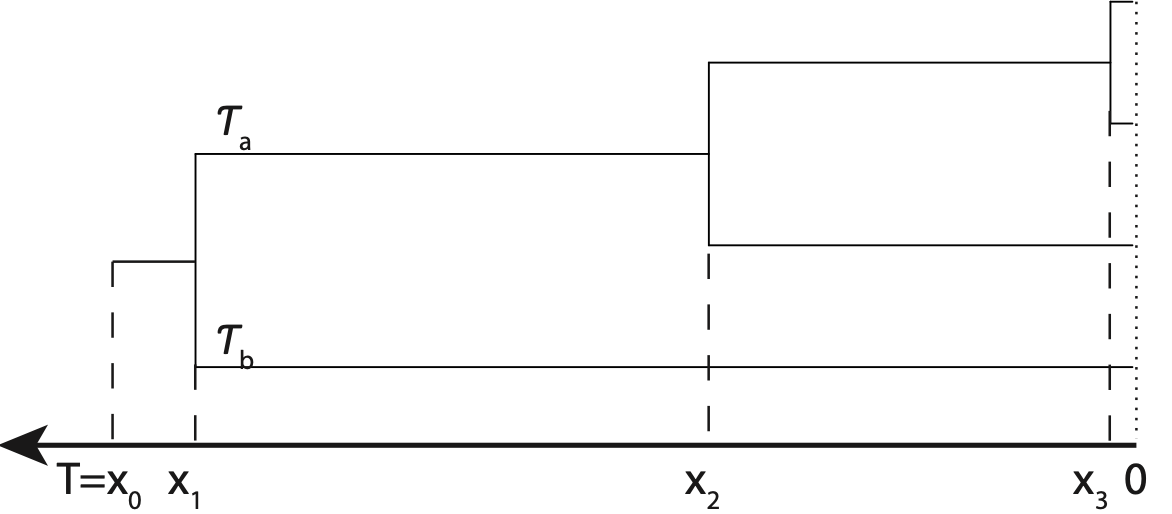
\includegraphics[width=1\linewidth, angle=0.0]{treepd.png}
\end{center}

With $p(T|x) = p(T|\rho = (\beta,\delta, T = x))$\\

If we calculate the probability $p(t,x_1)$ density of the branch between $t$ and $x_1$ we get. 

\begin{align*}
p(t+\Delta t, x_1) = \\(1-(\beta+\delta)\Delta t ) p(t,x_1) + 2\beta \Delta t p(t,x_1) p(0|t)    
\end{align*}

This leads to the following differential equation. 

\begin{align*}
    \frac{d}{dt}p(t,x_1) = -(\beta+\delta)p(t,x_1) + 2\beta p(t,x_1)p(0|t)
\end{align*}

Which is the same differential equation as for $p(1|t)$, but the initial condition differs. Here we have $p(x_1,x_1) = 1$. Thus for the solution we get. 

$$p(x_0,x_1) = p(1|x_0)/p(1|x_1)$$

For a tree of $n$ present day tips, age of the process $X_0$ and branching times $x_1, x_2,...,x_{n-1}$ we have the following probability density. 

\begin{align*}
p(T|x_0) = p(x_0,x_1)\beta p (T_a|x_1)p(T_b|x_1) =\\ \beta^{n-1} \prod_{i = 0}^{n-1} p (1|x_i)    
\end{align*}

An analogous strategy provides us with a tree probability density when $\rho < 1$ (indicating incomplete extant sampling) and $\phi > 0$ (sampling through time). 


\section{Coalescent Models}

While birth-death models allow the population size to vary stochastically, coalescent models instead treat the population size as a given. Thus the population size itself becomes a target of the inference.\\
A common assumption is that the underlying population dynamics are deterministic. 

\subsection{Wright-Fisher Process}

Is a model for the propagation of traits in a population of fixed size. It includes discrete generations where each generation consists of $N$ individuals.
\begin{itemize}
    \item Each individual in the offspring population chooses its parent uniformly at random from the $N$ parents.
    \item Thus a given parent has a binomially-distributed number of offspring. 
    \item For phylogenies of a particular gene, ploidy can be taken into account by multiplying $N$ by a factor which accounts for the number of copies of gene present in each individual. (e.g. for a diploid organism the number of gene copies is $2N$)
    \item The model assumes distinct non-overlapping generations and each member of a given generation has exactly one parent in the previous generation. 
    \item What these elements represent depends on the system of study; they might be genes or asexual organisms. \item The selection of the parent is completely random; the Wright-Fisher process is therefore neutral as fitness values are not considered.  
\end{itemize}

We want to determine the probability that the most recent common ancestor (MRCA) of two samples occurred at $m$ generations before the present. 

We consider the following. 

\begin{itemize}
    \item Since the parent of each individual is randomly picked, the probability that two individuals in the same generation have the same parent is $\frac{1}{N}$. 
    \item Thus the probability that two individuals in the same generation do not have a common ancestor in the previous generation is $\left(1-\frac{1}{N}\right)$. 
\end{itemize}


The probability that two sampled individuals first share a common ancestor in the $m^{\text{th}}$ generation before the present is the following. 

\begin{align*}
P_{\text{MRCA}(m)} = \underbrace{\left(1-\frac{1}{N}\right)^{m-1}}_{\text{No common ancestor in }\atop m - 1 \text{ generations}}\underbrace{\frac{1}{N}}_{\text{Common ancestor in the}\atop m^{\text{th}} \text{ generation}}   
\end{align*}

This results in a success probability of $1/N$. Since the mean of such a distribution is the inverse of the success probability we must wait on average $N$ generations to see a common ancestor of two samples from a population of size $N$. 

\begin{center}
    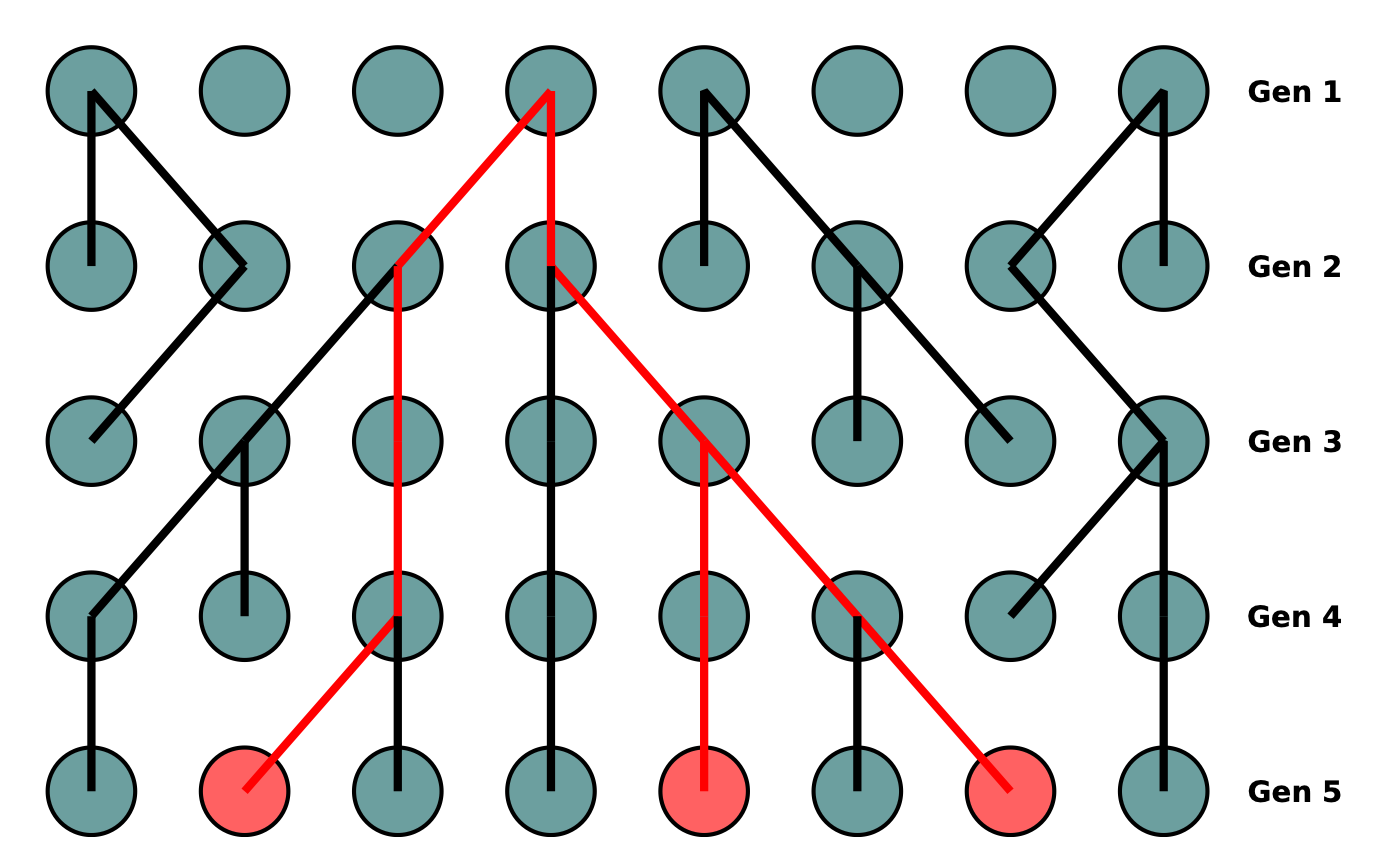
\includegraphics[width=1\linewidth, angle=0.0]{wfphylo.png}
\end{center}

\subsubsection{Coalescent in Calendar Time}

If $m$ is the number of generations let $g$ be the calendar time of a generation (e.g. 5 days). Therefore we we have the following for the calendar time span of $m$ generations. 

$$\Delta t = gm$$

In calendar time the probability density function for the coalescence of two lineages is the following 

$$pdf(N, \Delta t) = \frac{1}{gN}\text{e}^{-\frac{\Delta t}{gN}}$$

For large $N$ the time limit of the coalescence is exponentially distributed with mean $gN$.\\

If the number of samples $k$ is much smaller than the population size $N$ we have the following probability for a coalesence between any of the ${k\choose 2 }$ pairs. 

$$p_{\text{coal}} \approx {k\choose2}\frac{1}{N}$$


\subsection{Kingman's Coalescent}

Is a continuous-time Markov chain which produces time-trees. The process runs backwards in time by successive merging of events known as "coalesence".\\

If $N\gg k$ then it will produce the same tree as the Wright-Fisher model.\\

The times between coalesence events are drawn from an exponential distribution with rate parameters ${k\choose 2}\frac{1}{Ng}$. 

\begin{align*}
    P(\Delta t|N,g,k) = \exp{\left(-\Delta t {k\choose 2}\frac{1}{Ng}\right)}{k\choose 2}\frac{1}{Ng}
\end{align*}

We derive the average time for $n$ lineages to coalesce into one.

$$E[t_{root}] = Ng\sum^n_{k = 2}\frac{1}{{N \choose 2}}$$

Thus the mean time until all coalescent events happen is the sum over all probabilities in the tree. 

Coming from the previous equation we write the following. 

$$\sum ^n_{k =2} \frac{1}{{k \choose 2}} = \sum _{k = 2}^n\frac{2}{k(k-1)}$$

We can expand the term $\frac{2}{k(k-1)}$ to $\frac{2}{k-1}-\frac{2}{k}$ and get.

$$\sum _{k = 2}^n\frac{1}{{k \choose 2}} = \sum_{k = 1}^{n-1}\frac{2}{k}- \sum_{k = 2}^{n}\frac{2}{k} = 2(1-\frac{1}{n})$$

Therefore we find that $E[t_{\text{root}}] \rightarrow 2Ng$ as the number of lineages $n$. (i.e. number of leaves in the coalescent tree) becomes large. This is an upper bound on the expectation, while individual coalescent trees can be older than this.\\

\textbf{The Probability of a Coalescent Tree}

We calculate the probability of the following coalescent tree.

\begin{align*}
    P(T|Ng) = \overbrace{\exp(-\Delta t_1{4 \choose 2}\frac{1}{Ng})}^{\text{Nothing happens}\atop\text{in }\Delta t_i}\times \overbrace{\frac{1}{Ng}}^{\text{Probability of particular}\atop \text{coalescent event}}\times\\ \exp(-\Delta t_2{3 \choose 2}\frac{1}{Ng})\times \frac{1}{Ng} \times\\ \exp(-\Delta t_3{2 \choose 2}\frac{1}{Ng})\times \frac{1}{Ng} = \\
    \prod_{i = 1}^{n-1}\exp\left(-\Delta t_i  {k_i \choose 2}\frac{1}{Ng}\right)\frac{1}{Ng}
\end{align*}

\begin{center}
    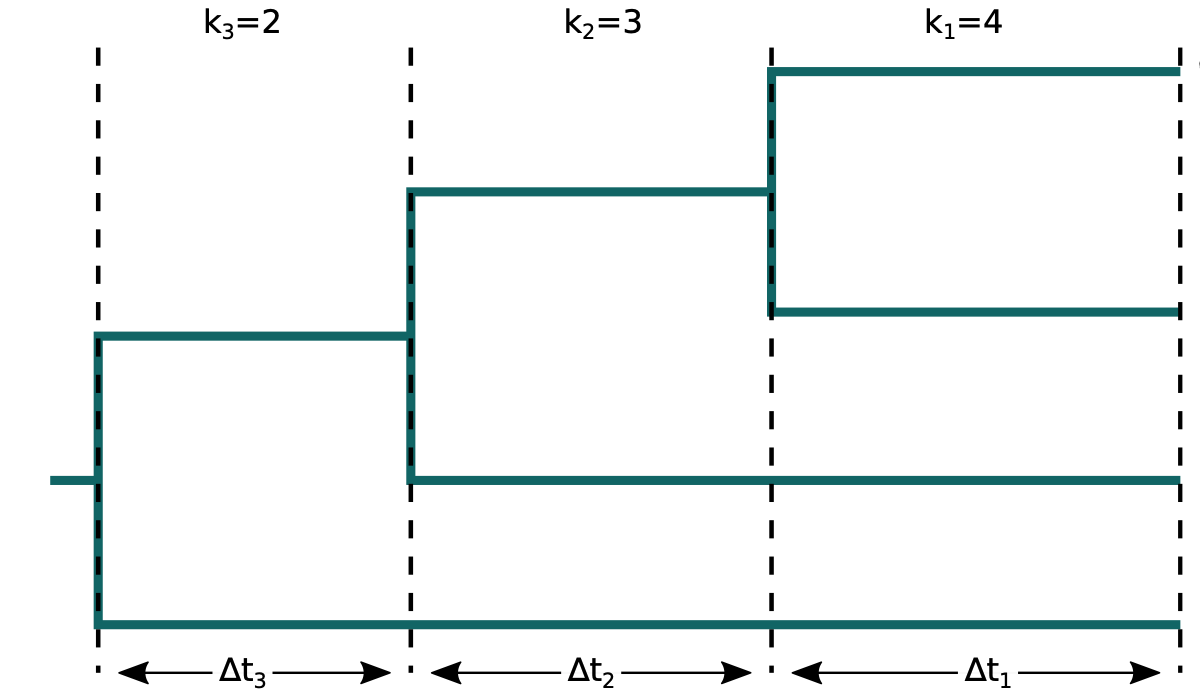
\includegraphics[width=1\linewidth, angle=0.0]{coaltree.png}
\end{center}

\begin{itemize}
    \item If we take a real tree (inferred from genetic data sampled from a real biological population) and infer population size the result might be biased sine the real dynamics differ from Wright-Fisher dynamics
    \item Real populations are structured while Wright-Fisher populations are completely homogeneous.
    \item The coalescent process is often derived as a limit of the Wright-Fisher process as done here and appears as the limit of many other population processes. $\rightarrow$ Thus the coalescent is believed to be fairly robust.  
\end{itemize}

\textbf{General Assumption of the Coalescent}

\begin{enumerate}
    \item Samples are members of a population that is at \textbf{demographic equilibrium}, which justifies the use of fixed or slowly varying population sizes. 
    \item \textbf{Small sample number} compared to the total population size, which justifies the neglection of more than two lineages coalescing at the same time. 
    \item Populations are \textbf{"well-mixed"}, thus samples are drawn uniformly at random, which justifies the coalescent rate between any pair of sampled lineages being equal. Population structure violates this assumption.
\end{enumerate}

\textbf{Extension of Population Size Changes}\\

$P(T|N(t))$ is calculated via the rate of coalescence $\frac{1}{N(t)}$, where $N(t)$ is the population size as a function of time $t$. For large population sizes we have a slower coalescence rate.\\

Under a Wright-Fisher model with varying population size the probability of a sampled tree becomes. 

\begin{align*}
    P(T|N(t)) = \prod _{i = 1}^{n-1}\exp \left(-\int_{t_i}^{t_{i+1}}{k_i \choose 2}\frac{dt}{N(t)g}\right)\frac{1}{Ng}
\end{align*}

For a given parametric form e.g. $N(t) = N_0\exp(-\gamma t)$ the model yields the likelihood for the given demographic model parameters. This allows us to directly test different demographic scenarios for a given tree.\\

\textbf{Non-parametric Population Dynamics}\\
We assume that the population has distinct constant sizes in each interval between coalescent events. We can obtain a separate maximum likelihood estimate for each population size. 

\subsection{Coalescent Approximation of Birth-Death Models}

We can develop coalescent distributions that approximate the probability density of sampled phylogenies generated by birth-death processes.\\

We assume that the ODE approximation $I(t) = I(T)\exp((\beta -\delta)(T-t))$ holds. Birth events occur at time $t$ with the rate $\beta I(t)$ where $I$ is the number of individuals. Every birth is a potential coalesence between sampled lineages and the probability of choosing a sampled lineage pair is ${k \choose 2}/{I(t)\choose 2}$ and the approximate coalesence rate is $\beta I(t) \frac{k(k-1)}{I(t)(I(t)-1)}\approx {k \choose 2}\frac{2\beta}{I(t)}$.\\

The quality of the approximation heavily depends on how well birth-death population dynamics are approximated by the deterministic ODE solution. The approximation can perform very poorly if the population size is small, as it is always the case when an epidemic starts. 

\subsection{Comparing Birth-death models to Coalescent Models}

These models are used to probabilistically relate a populations demography to its phylogenetic history. Both allow for inference of demographic and epidemiological parameters but may differ in their parametrization. 

\textbf{Birth-death Models}\\
\begin{tabular}{|l|l|}
\hline
\textbf{Advantages}                                                                                        & \textbf{Disadvantages}                                                                                  \\ \hline
\begin{tabular}[c]{@{}l@{}}Accounts for\\ stochastic\\ variability in\\ population\\ dynamics\end{tabular} & \begin{tabular}[c]{@{}l@{}}Sensitive to\\ unmodeled \\ changes in \\ sampling \\ fractions\end{tabular} \\ \hline
\begin{tabular}[c]{@{}l@{}}Easier \\ interpretation of \\ parameters\end{tabular}                          & \begin{tabular}[c]{@{}l@{}}Difficult to \\ extend to\\ complex \\ population \\ models\end{tabular}     \\ \hline
\begin{tabular}[c]{@{}l@{}}Uses sampling \\ information\end{tabular}                                       &                                                                                                         \\ \hline
\end{tabular}

\textbf{Coalescent Models}\\

\begin{tabular}{|l|l|}
\hline
\textbf{Advantages}                                                                          & \textbf{Disadvantages}                                                                                               \\ \hline
\begin{tabular}[c]{@{}l@{}}Fast likelihood\\ calculations\end{tabular}                       & \begin{tabular}[c]{@{}l@{}}Sensitive to \\ uncertainty in \\ population \\ dynamics at \\ high sampling\end{tabular} \\ \hline
\begin{tabular}[c]{@{}l@{}}Easy to extend\\ to complex \\ population\\ dynamics\end{tabular} & \begin{tabular}[c]{@{}l@{}}Sensitive to\\ hidden\\ population \\ structure and \\ nonrandom\\ sampling\end{tabular}  \\ \hline
\begin{tabular}[c]{@{}l@{}}Accounts \\ naturally for\\ incomplete \\ sampling\end{tabular}   &                                                                                                                      \\ \hline
\end{tabular}

\section{Bayesian Inference}

There are two main approaches to statistics, the frequentist approach and the Bayesian approach. In a frequentist view we see probabilities as relative frequencies of outcomes of repeatable random experiments (e.g. dice roll). Thus probabilities are only assignable to repeatable experiments and they are treated as an intrinsic property of the system. Furthermore, under this view the inference of model parameters is treated as fundamentally different from the prediction of outcomes.\\

The Bayesian approach on the other hand sees probabilities as plausibilities of propositions conditional on available information. Under this view probabilities are assignable to any unambiguous proposition and they represent a lack of information to predict the outcome with certainty. Here the inference of model parameters is treated in the same way as the prediction of outcomes. 

\subsection{Inference of Genetic Distances}

We have a Jukes-Cantor model for the likelihood of the alignment with $S = 4$ substitutions given the total number of sites $L = 10$ and the distance $d$. 


\begin{align*}
P[S|d,L] =& \left[ \frac{1}{4} + \frac{3}{4}\exp \left(-\frac{4}{3}d\right)\right]^{L-S} \\ \times & \left[ \frac{1}{4} - \frac{1}{4}\exp \left(-\frac{4}{3}d\right)\right]^{S}
\end{align*}

Thus under our model we can say that the number of segregating sites follows the likelihood $P(S|d,L,M)$. Under a Bayesian viewpoint we can talk about the probability of a certain distance $d$ given the substitutions, the length and the model, thus we have $P(d|S,L,M)$. To find $P(d|S,L,M)$ we use Bayes rule. 

$$P(d|S,L,M) = \frac{P(S|d,L,M)P(d|L,M)}{P(S|L,M)}$$

Where $P(d|L,M)$ quantifies knowledge of $d$ in the absence of the observation $S$. $P(S|L,M)$ is the distribution over possible number of segregating sites $S$ given the JC69 model and any independent $d$.\\
Here we assume that our prior information is $0\leq d \leq 3$. 

$$    \begin{cases}
      \frac{1}{3}, & \text{if}\ 0\leq d \leq 3 \\
      0, & \text{otherwise}
    \end{cases}$$

This yields a probability distribution with $L_{max} = 0.7$.\\

If new data is acquired we can update this estimate using Bayes. We have a new alignment with $(L' = 90, S' = 48)$. Thus we update our estimate by using the previously calculated posterior as our new prior.\\

\textbf{This is equivalent to inferring $d$ from both data sets simultaneously.}

\begin{center}
    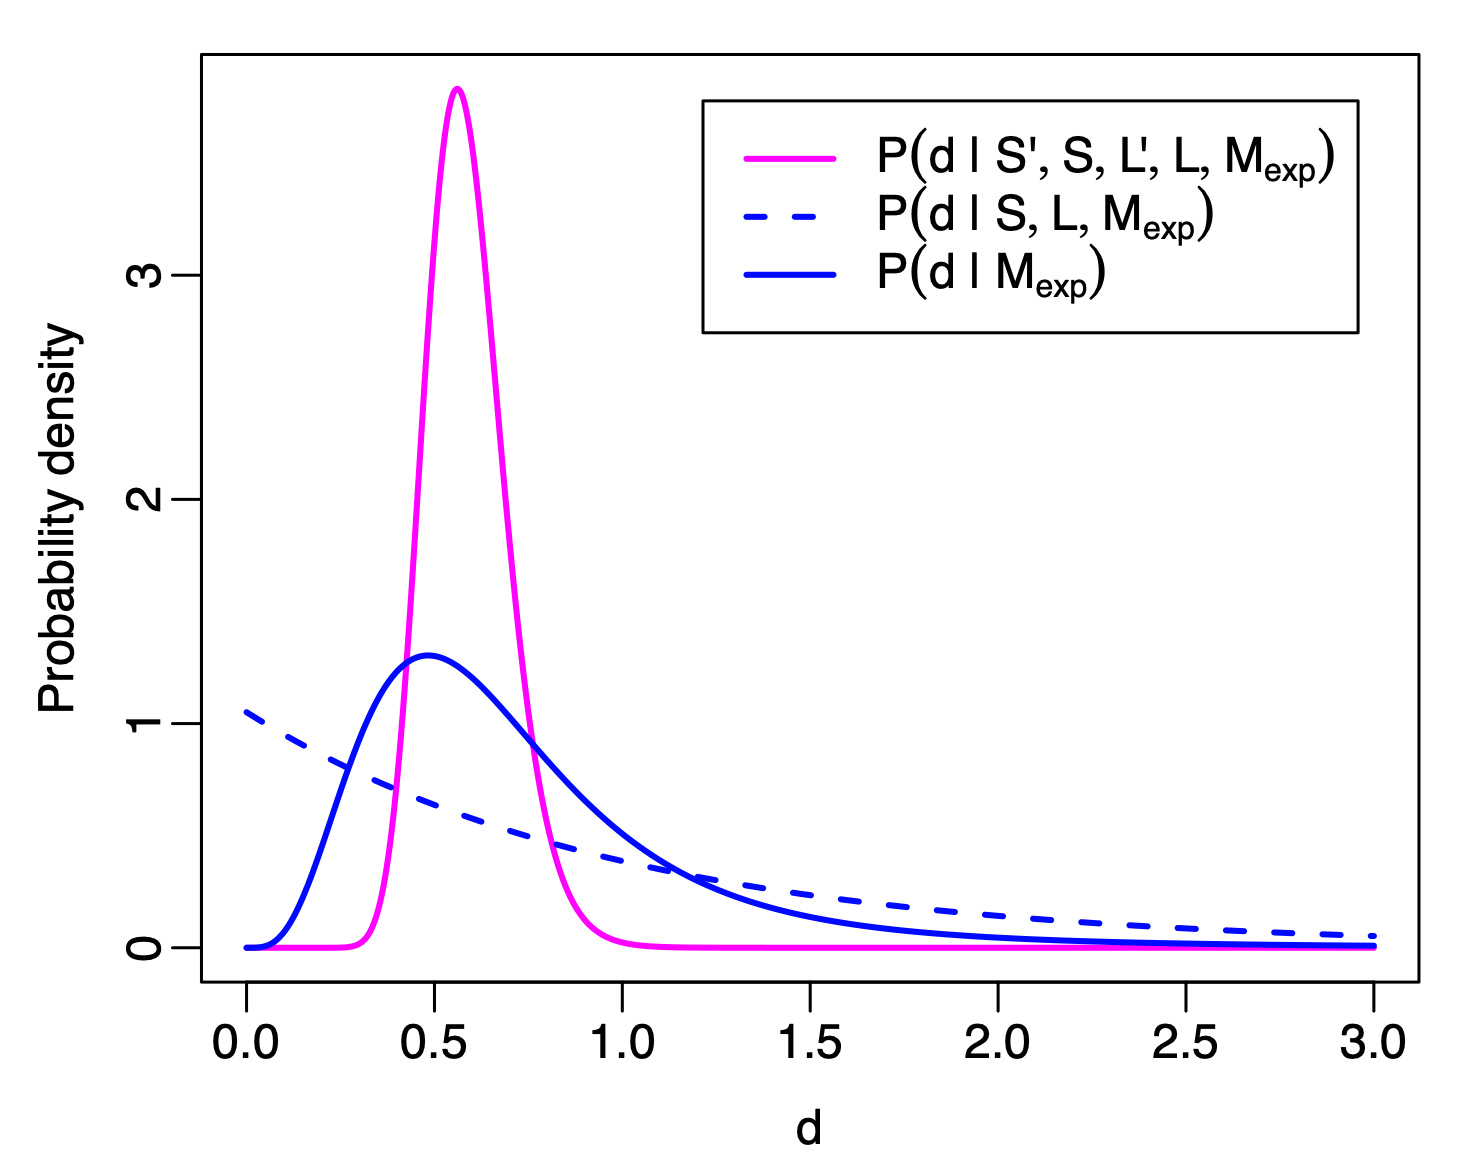
\includegraphics[width=1\linewidth, angle=0.0]{bayesprior.png}
\end{center}

\begin{mdframed}[backgroundcolor=astral] 
    \textbf{Credible Intervals}\\
    The 95 \% credible interval is an interval of the posterior distribution containing 95 \% of the probability. We ignore the 2.5 \% of the sample on both sides. The interval is often chosen, such that it has the smallest size, this is called the highest posterior density (HPD).
    
    \begin{itemize}
        \item The 95\% HPD can also be found by lowering a threshold density under the curve where the density exceeds the 95 \% threshold. 
        \item The interval can be interpreted as \textbf{the probability of an unknown value falling into this region is 95 \% given the data.}
        \item This is different from a 95 \% \textbf{confidence interval} which is the truth-containing interval 95\% of the time when averaging over all possible data sets.  
    \end{itemize}
\end{mdframed}

\subsection{Difficulties of Bayesian Inference}

Bayes' Law is given by the following formula. 

$$P(\theta|D,M) = \frac{P(D|\theta,M)P(\theta|M)}{P(D|M)}$$

In practice it is often difficult to determine the denominator $P(D|M)$ of this equation, this term can be seen as a normalizing constant for the posterior distribution. 

$$P(D|M) = \int P(D|\theta,M)P(\theta|M)d\theta$$

This integral is often not numerically solvable if $\theta$ has many dimensions, which is true for most phylogenetic and phylodynamic problems. 

Thus we use Monte Carlo methods. 
\begin{itemize}
    \item Algorithms which produce random samples of values in order to characterize a probability distribution. 
    \item Markov Chain Monte Carlo is an example of such an approach which is used very often for phylogenetic and phylodynamic problems.
\end{itemize}

$\rightarrow$ See the excellent article on Wikipedia.

\url{https://en.wikipedia.org/wiki/Metropolis-Hastings_algorithm}\\

In Bayesian phylogenetics, we take samples from the posterior distribution in order to characterize the probability distribution of the tree $T$.\\

The MCMC algorithm relies on the use of appropriate proposal distributions that allow the Markov chain to probe the parameter space efficiently.\\

Here we want to calculate the probability of a given tree $\tau$, the substitution model parameters $Q$ and $\eta$ which are the parameters of our phylodynamic model.

$$P(\tau, Q, \eta|A) = \frac{1}{P(A)} P(A|\tau, Q)P(\tau|\eta)P(Q,\eta)$$

$P(\tau|\eta)$ is the prior of our tree and $P(Q,\eta) = P(Q)P(\eta)$ are the parameter prior distributions.\\

This Bayesian approach has the following characteristics. 
\begin{itemize}
    \item Joint inference of the phylogenetic tree, the substitution model parameters and the phylodynamic model parameters. 
    \item Accounts for uncertainty in the tree and in the model parameters. 
    \item It allows us to include additional sources of information such as constraints on the tree topology.
    \item The resulting posterior distribution naturally includes the uncertainty. 
\end{itemize}

Here we assume that sequence evolution is neutral due to way we factorized the joint probability for the tree and the model parameters (Tree generation is separate from sequence evolution).

The MCMC algorithm proposes new state $\tau ', \theta ', \eta '$ based on state $\tau ', \theta ', \eta '$ and evaluates the numerator of Bayes formula. Here the new tree is proposed using tree-space proposal distributions. The other parameters are scalars and can be proposed via random scaling, random walks, etc.\\

$\rightarrow$ Acceptance/Rejection of the new state leads to a set of the accepted states which is s sample from the posterior distribution $P(\tau, Q, \eta|D)$.
\subsubsection{Tree Space Proposal Distributions}

We want get a proposal distribution from the whole space of rooted time trees. Thus to get the proposal distribution $q_i(\tau'|\tau)$ we generate new random trees using the following methods. 

\begin{center}
    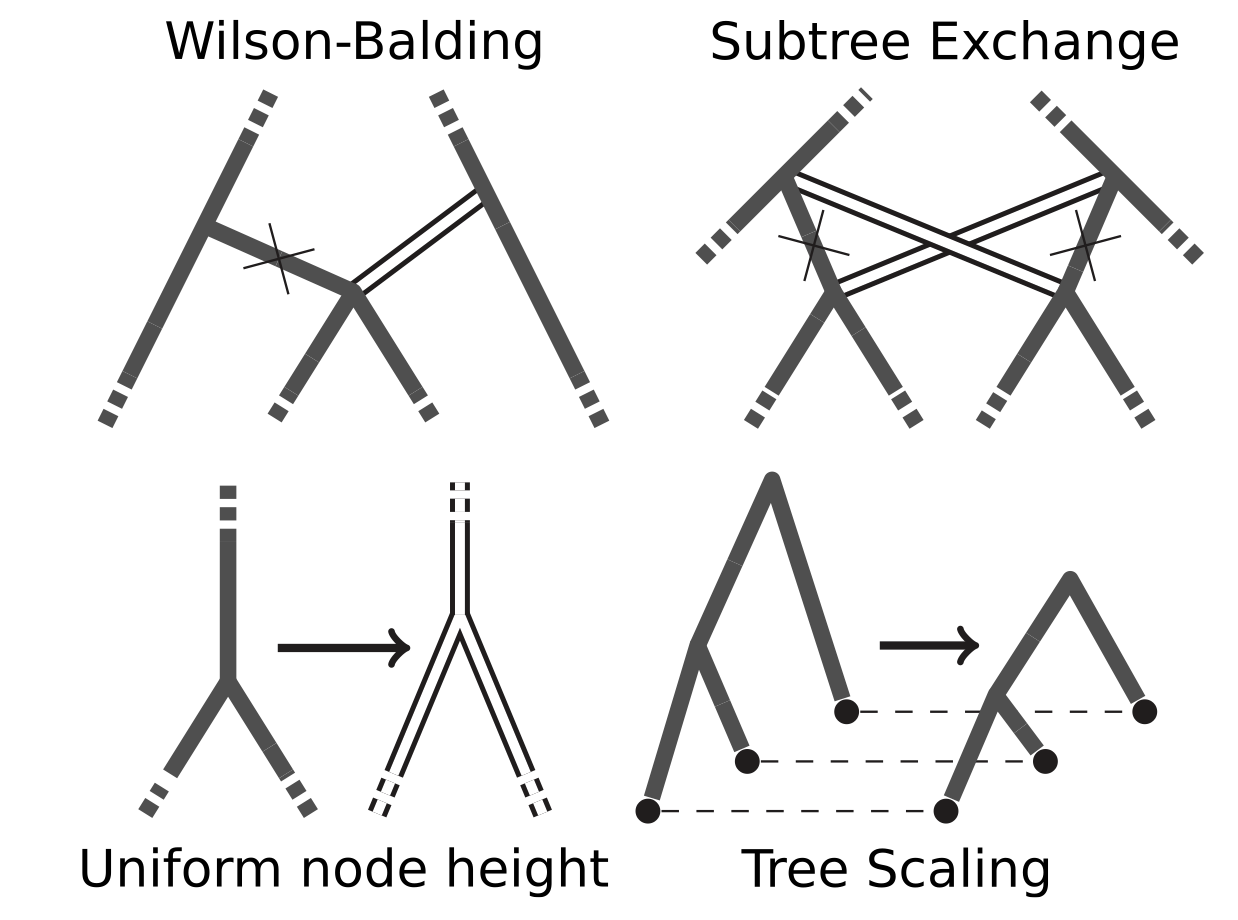
\includegraphics[width=1\linewidth, angle=0.0]{treeproposal.png}
\end{center}

\begin{itemize}
    \item \textbf{Wilson-Balding}: A branch swapping move proposed by WILSON and BALDING 1998 which involves removing a subtree and re-attaching it on a new parent branch
    \item \textbf{Subtree Exchange}: Two subtrees are randomly swapped. \item \textbf{Uniform Node Height}: Randomly selects true internal tree node (i.e. not the root) and move node height uniformly in interval restricted by the nodes parent and children.
    \item \textbf{Tree Scaling}: Scale the branch length of a tree proportionately. {\color{red} CONFIRM}
\end{itemize}

\section{Phylodynamic Applications}

\subsection{Structured Populations}

Populations often have some internal structure such as geographical separation between parts of the population. 

\begin{mdframed}[backgroundcolor=astral] 
    \textbf{Population Structure}\\
    A population is structured if its members possess one or more traits (e.g. location, group membership, etc.) that affects their phylodynamic parameters such as birth rate, death rate, sampling rate or coalescence rate. 
\end{mdframed}

\textbf{Spatial/Geographic Structuring}

Gene flow between subpopulations can be limited due to geographic separation. How strongly this impacts phylodynamic parameters depends on the rate of migration (relative to the local birth rate) between subpopulations.\\

\textbf{Non-spatial Structuring}

Spatially mixed populations can be mixed, this is often the case in pathogen populations which are composed of within-host sub-populations. Some sub-populations may show traits such as drug resistance which have a strong influence on the reproductive success.\\

Individuals of the population may be in different epidemiological states (e.g. exposed vs infectious). \\

Sampled animals may even be members of different species, between which there has been horizontal gene transfer, although this is very rare.\\

\textbf{Population structure can be an important factor in shaping the phylogenetic relationships between samples.}

\begin{center}
    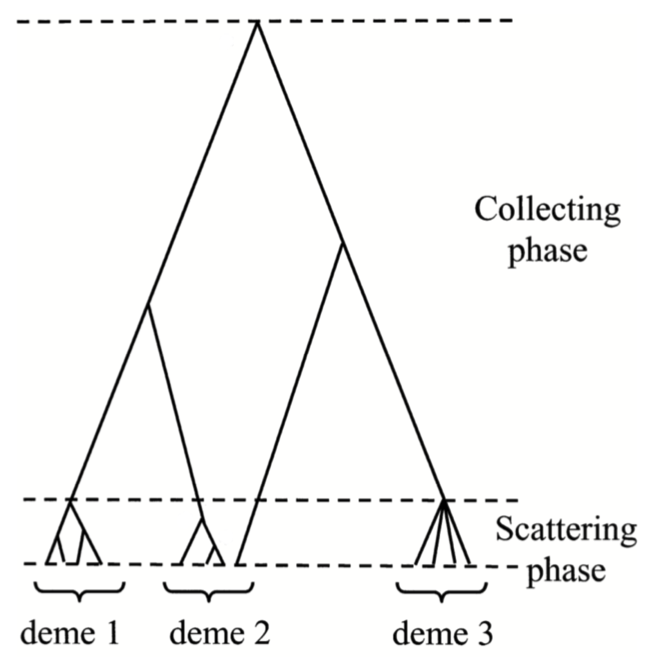
\includegraphics[width=0.7\linewidth, angle=0.0]{demephylo.png}
\end{center}

$\rightarrow$ Here the coalesence rate within the demes (a local group of individuals, i.e. from the same taxon, that interbreed with each other and share a gene pool) is much higher than in between the demes.\\

If one fails to account for such structure there is a risk that the results will be biased. We can use structure aware phylodynamic models to account for such biases. 

Incorporating structure into phylodynamic models also allows us to directly address questions relating to population structure. We can consider questions regarding the migration rate between islands or find information regarding the sizes of sub-populations. Even questions about when a disease entered a geographic location can be answered. 

\textbf{Example}

Consider a population of individuals of which some are sensitive to some drug and others are not. When sampling from the population we do not know about the history of the lineages but only about their current resistance status. Thus if we reconstruct the tree, the history of how the resistance was transmitted will be missing. However if we find many clustered leaves then it is very likely that the drug resistance was transmitted; if the resistance occurred de-novo many times then drug-resistant and drug-sensitive tips will be mixed. 

\subsection{Structured Birth-Death Models}

We extend the birth-death model to include individuals of different types and transitions between them. 

\section{Phylogenetic Networks}
\end{multicols*}
\end{document}
